% !TeX root = ../thuthesis-example.tex

\chapter{Methodology}

\section{Motivation}

As we have established previously, it is difficult to control the generated adversarial patterns with existing methods. 
By control here we mean a possibility to lead our generation to a particular direction according to the attacker's will, thus being able to generate a wide range of possible patterns.
So, the main idea of our methodology is to use the remarkable generative abilities of diffusion models to produce natural-looking adversarial clothes.
Moreover, since we want our method to be zero-shot, that is, to use pretrained models only, ideally, we would like to be able to use the DM to find a trajectory that would lead us to adversarial samples hidden inside the areas of distribution of natural-looking images.
Here, trajectory denotes the denoising path the DM choses when gradually producing the final result starting from random noise. 
So, we would like to be able to change the default generation trajectory of our DM to push it towards enhancing the adversarial effects of the image.
% todo more 

\section{Pipeline}
\subsection{Introduction: Quick Overview}

We have two models involved in the pipeline: a diffusion model and a detector model.
As input, we receive a prompt from the user, and as output, we have to generate adversarial clothes with a pattern as close to the original generation of our stable diffusion model as possible.
Again, in our case, adversarial means that the clothes can help to avoid being detected altogether instead of just making the detector assign an incorrect class to the detected bbox.
At the same time, we also need to ensure that the generated pattern is still effective in the physical world, since our ultimate goal is to be able to print the clothes, put them on and demonstrate how they can be used to avoid detection systems.

First, we generate a latent that would correspond to the input image according to our diffusion model.
This latent can be either random or somehow modified according to the user's wishes. 
Again, one of the main advantages of our method is that, unlike other methods, it is able to trade adversarial effectiveness off in order to create natural-looking patches that can be controlled by the user with the use of prompt and initial conditioning, which is the chosen latent, our starting point in the noise distribution.
It is essential that the prompt makes sense according to whatever the user is trying to generate.
That is, even if the user was to only provide the initial latent, they still need to ensure that the prompt does not contradict the task, and rather help to push the generation into the right direction.

After that, we modify the sampling process of the diffusion model, adding ``detector guidance'' to the update in order to ensure that our patch helps us avoid the detector.
In order to obtain this ``detection guidance'', we unfold the latents into the corresponding patch and create clothes that are used in a chosen pipeline to estimate the efficiency of our detector, and change the update direction based on the detector's output.
Here, we have used two types of pipelines for calculating detection guidance: 2D and 3D.

Other guidances, like the ``fixation guidance'', are also used to ensure the naturalness of our final generation.

In the end, we once again obtain the final image from the latents and make adversarial clothes out of them using the same strategy.

\subsection{Models}

In order to understand the pipeline in more detail, first, we need to look at the component parts closely.

Two models are used in this pipeline: a Stable Diffusion model (SD) for generating the patch, and a YOLOv2 model (YOLO) to ensure that the generated patch is adversarial with respect to detection.
Naturally, it is also possible to choose other diffusion and detection models.
We stopped at SD mainly because of its speed and large variety of results, while YOLO was chosen to compare against other baselines as one of the most widely used models.

All weights of the models involved in the process are frozen, but the latents that are used and optimized by the SD have their gradients unlocked in order to enable adversarial guidance.

\subsubsection{Stable Diffusion}
% TODO details on SD

\begin{figure}[ht!]
\centering
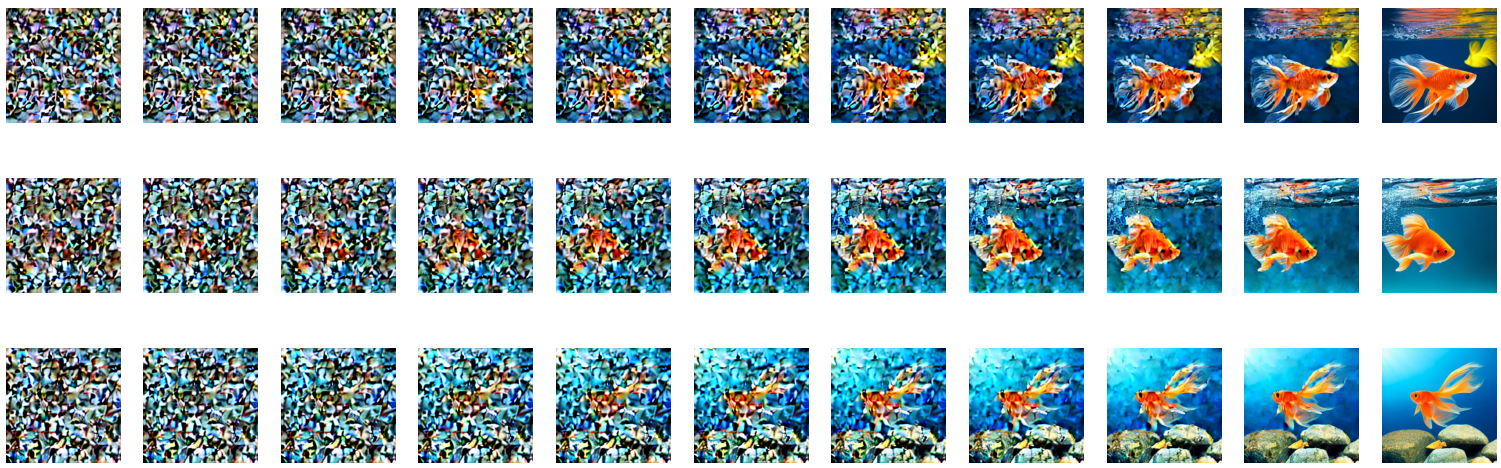
\includegraphics[width=150mm]{figures/sd_example_gf.png}
\caption{Example of a Stable Diffusion (MiniSD) generation. Prompt: ``A beautiful goldfish swimming through the ocean''. 50 steps, each 5th step drawn, three random noises used as starting points for the rows.}
\label{sd_generation_example}
\end{figure}

\paragraph{Introduction} On a high level of understanding, a pretrained SD model, just like any other DM, generates trajectories from the noisy space to the meaningful for us humans space by gradually removing noise from this random starting point. 
Figure~\ref{sd_generation_example} demonstrates three examples for such trajectories for the SD model that was used in this work.
The prompt is fixed for all these examples: ``A beautiful goldfish swimming through the ocean''.
The first column depicts three random noises that were used as starting points for the corresponding three trajectories that show the denoising process.
In this process, as we look at the pictures in each row from left to right, we observe the model gradually remove the noise to arrive at different finishing points. 
All three final generations in the last column, however, satisfy our conditioning requirement, which is the given prompt.

So, during the training process of a DM, noise is added to input images, and the main part of the model, normally its U-Net component, is training to predict the noise that was added at each step.
That way, during sampling, we are able to use this pretrained U-Net to go in the opposite direction of removing noise. 

Another important part of the process is conditioning, which in case of a SD model is usually added in the form of a text prompt, or more rarely a semantic map.
The conditioning is inserted into the U-Net with the use of attention, and the text itself is encoded with a CLIP model. 

Finally, a SD model is a latent diffusion model. 
Since we often want to work with large images that might take too much GPU memory, this class of models works on optimization in a latent space instead of the original pixel space of actual images. 
In order to work in this space, however, we have to be able to go into the space and leave it at will.
Typically, a Variational AutoEncoder (VAE) model is used for this purpose: its encoder allows the transition into the latent space, while its decoder returns latents to the corresponding images in the real pixel space.



\begin{figure}[ht!]
\centering
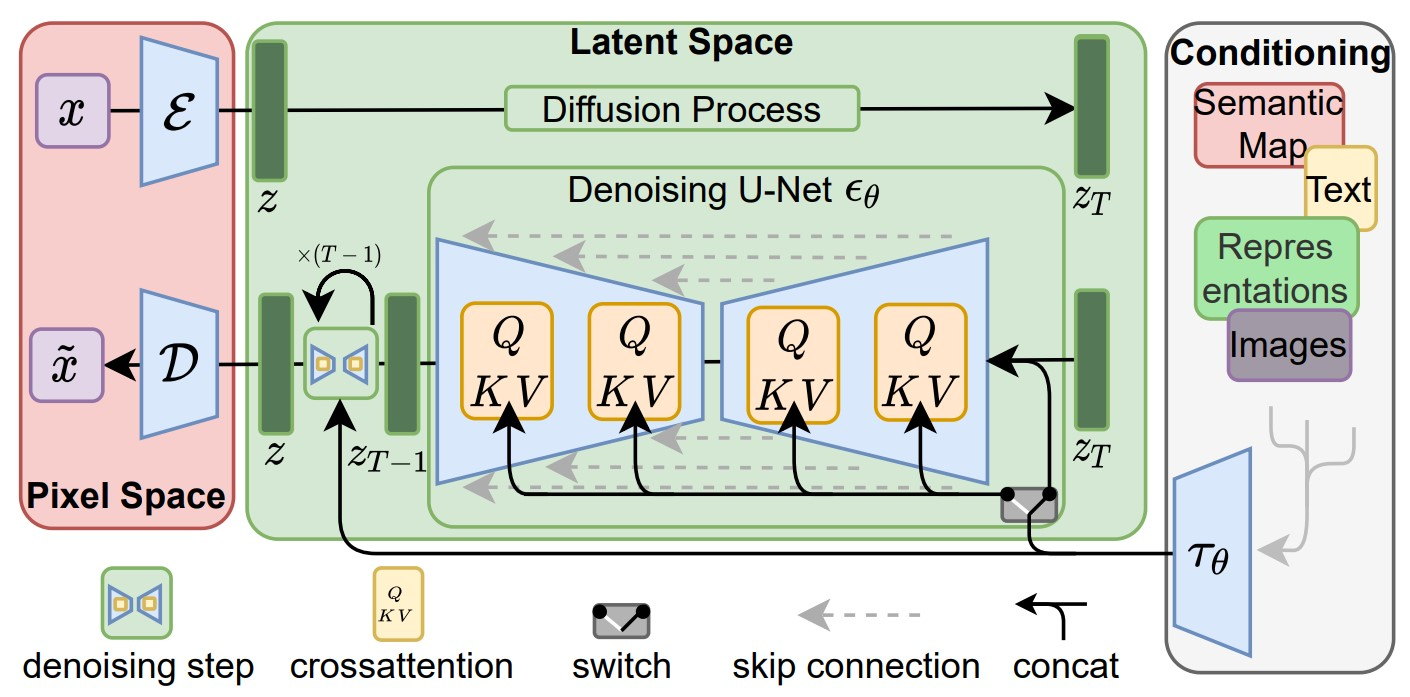
\includegraphics[width=120mm]{figures/sd.jpg}
\caption{Stable Diffusion Training Pipeline.}
\label{sd}
\end{figure}

\paragraph{Formalization} Now, let us turn to a little more low-level explanation with formulas and illustrations.

Figure~\ref{sd} depicts the pipeline in the scheme from the original paper~\cite{stable_dif}.
The leftmost red part indicates the pixel space with real images, and the green part---the training process that is happening in the latent space.
The transitioning between the spaces is possible with the use of a VAE with encoder $\mathcal{E}$ and decoder $\mathcal{D}$.
That is, a real image $x$ can be translated into a latent $z$ in the latent space by applying the encoder $\mathcal{E}$ of this VAE, while the reverse process is carried with the decoder $\mathcal{D}$: 
$$z = \mathcal{E}(x), \Tilde{x} = \mathcal{D}(z)$$

$\Tilde{x}$ is a reconstructed original image $x$. 
During training of a SD, the weights of its VAE model are fixed.

The forward diffusion process gradually adds noise to our original latent $z$ in $T$ steps, and the model trains to predict the previous latent $z_{t-1}$ for all $z_t$.
So, our SD is actually learning the original data distribution by learning how to reverse a fixed Markov Chain of length $T$.
A denoising U-Net model $\epsilon_\theta$ is used to predict the noise that can be used to obtain $z_{t-1}$.
The text prompt is included in the U-Net with help of cross-attention as shown on the picture: or conditioning $y$ is turned into its representation $\tau(y)$.
% TODO should I include the loss function for SD?

After training is completed, we obtain a U-Net model that can denoise our latents.
During sampling, we take a prompt and an initial latent, be it random or somehow conditioned, and then run the trained U-Net for several iterations to denoise it, apply our decoder $\mathcal{D}$ and obtain our final image $\Tilde{x}$.
Theoretically speaking, each iteration in the denoising sampling cycle improves our final result; in practice, however, for a simple generation without specific guidances, a relatively small number of iterations ($\lesssim 1e2$) is enough to obtain a meaningful realistic result.
On the contrary, since generation is performed with a fixed scheduler, it is impossible to run the cycle for an infinite number of iterations without altering the sampling process of the given pretrained model.

\paragraph{Guidance}\label{sec:guidance}
Apart from conditioning, there exist other methods that push the generation towards a particular desired direction.
Let us formally describe guidance, a method that can be used to ensure that our generated image is not random in the space of all generations that satisfy the prompt, but rather is somehow altered.
Let us take a look at the update formula for the latents in the diffusion sampling cycle in the simplest form starting from $z_T \sim \mathcal{N}(0, 1)$:
$$\hat\epsilon_t = \epsilon_\theta(z_t;t,y)$$

where $z_t$ is the latent at step $t$ and $y$ is our condition, typically a prompt.
As we have previously stated, in this formula, we are predicting an estimate of the noise that was added to $z_{t-1}$ in order to create $z_t$:
$$z_{t-1} = \text{scheduler}(z_t, \hat\epsilon_t, t)$$

where scheduler depends on our sampling method; our SD uses pseudo numerical methods for diffusion models.

% TODO talk about classifier guidance? 

It was, however, proven that for improving the quality of the image and for a better conditioning it it better to use classifier-free guidance~\cite{ho2022classifierfree}:
$$\hat\epsilon_t = (1+s)\epsilon_\theta(z_t;t,y) - s\epsilon_\theta(z_t;t,\emptyset)$$

where $s$ is a hyperparameter that determines the strength of classifier-free guidance and is typically set to 7.5.
Without this guidance, the conditioning is rather poor and the result might not correspond to our prompt well.
Let us also recall that since DMs in general are score-based, $\epsilon_\theta(z_t)$ estimates the score function for the intermediate noisy distributions between $z_t$ and $z_{t-1}$:
$$\epsilon_\theta(z_t) \approx -\sigma_t\nabla_{z_t} \log p(z_t)$$

Now we can take a look at sampling even in a more general light and learn how to add the an arbitrary guidance to the formula:
$$\hat\epsilon_t = (1+s)\epsilon_\theta(z_t;t,y) - s\epsilon_\theta(z_t;t,\emptyset) + v\sigma_t\nabla_{z_t}g(z_t; t, y)$$

here, $g$ can be any energy function that guides our generation in a meaningful way, $v$ is self-guidance weight and $\sigma_t$ converts the score function to a prediction of $\epsilon_t$.

\paragraph{MiniSD} It is also important to note that due to our GPU resources limitations, we were unable to use the standard SD and used MiniSD from Hugging face instead; compared to its standard version, the MiniSD can generate images at resolution 256 without a noticeable loss in quality.

\subsubsection{YOLO}

\begin{figure}[ht!]
\centering
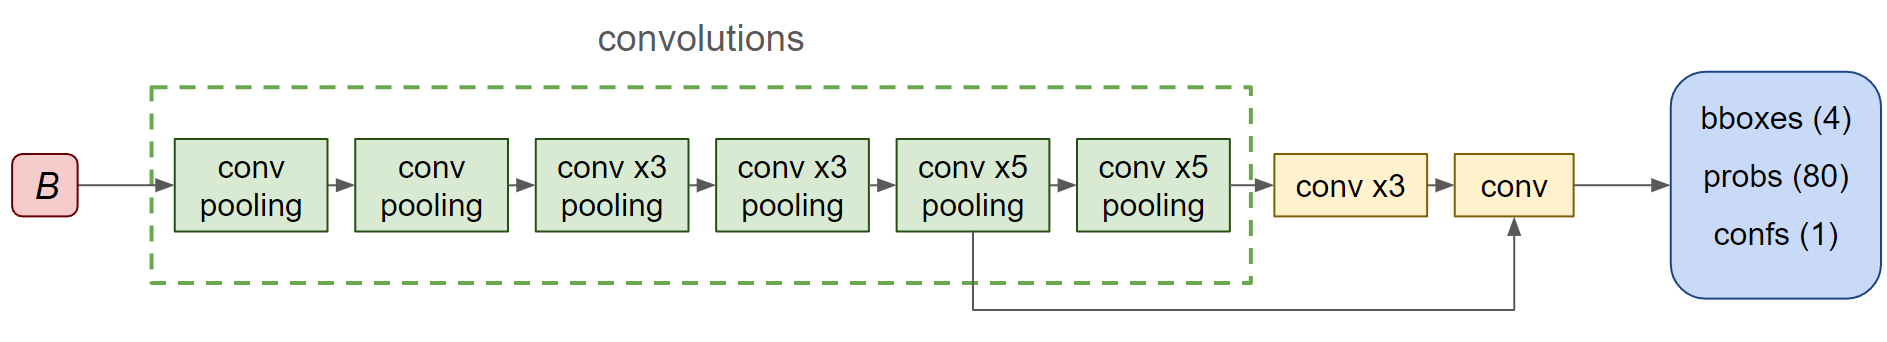
\includegraphics[width=150mm]{figures/yolov2.png}
\caption{Darknet-19, detection pipeline.}
\label{darknet19_detection}
\end{figure}

Another important model that we use in our pipeline is YOLO.
Figure~\ref{darknet19_detection} shows the architecture of the Darknet-19 that was introduced in the paper as a model that can be used for classification and detection. 
More specifically, in general, only the green part of the scheme is Darknet; the depicted architecture is a Darknet modification that is used for detection. 
When the yellow follow-up convolutions are replaced with another single convolution, the model becomes its classification Darknet-19 modification; they are trained jointly in the original paper.

The pipeline itself is very simple. 
In the simplest case, for a detection Darknet, a batch of square input images $B$ of size $3\times 416\times 416$ goes through the convolutions and poolings until the final predictions are obtained.
As it has been mentioned previously, the output data of YOLO consists of three parts: bboxes that show the positions of the predictions, probabilities for all classes, and confidences in predictions. 
Since each bbox is defined through its position and size, all of them are predicted in four values.
YOLOv2 specifically was trained for the COCO dataset~\cite{cocodataset}, the Darknet model returns probabilities for 80 classes. 
The confidence, or the objectiveness score, predicts the IoU between the proposed bbox and the ground truth label. 
The architecture also contains a shortcut as shown on Figure~\ref{darknet19_detection} to make the model take fine-grain features into consideration.
Each convolutional layer in the scheme is followed by batch normalization as regularization to speed up convergence and stabilize the training process. 

Another trick that is used in YOLO is anchors. 
After the batch of images $B$ goes through all the convolutions, we obtain feature maps for the images of size $13\times 13$, which can be understood as positions on the images. 
For each of these positions, our model learns to predict offsets for $5$ anchors that denote most cluster centers for object sizes of training dataset. 
That is, the authors chose the number of clusters for all object sizes in the training data as $5$ (the number chosen empirically), and then, instead of actually predicting the size of the object in the grid, we predict offsets to these anchors; centers of objects, that is, their positions, are also predicted as offsets from the central positions in the grid.
So, to sum up everything that has been mentioned, the final output has size $\text{batch\_size}\times 13 \times 13\times 5\times (4 + 1 + 80)$.

% TODO details on YOLO?

\subsection{General Pipeline}

In this section, we will introduce the general pipeline we used for our adversarial generations.

\begin{figure}[ht!]
\centering
\subcaptionbox{Original SD\label{sd_my-a}}{
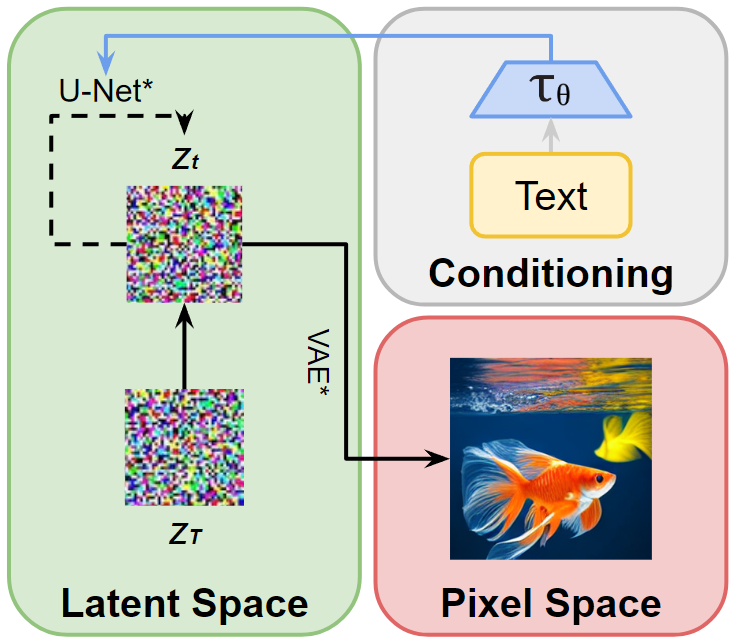
\includegraphics[width=0.45\linewidth, trim={0 0 0 0}]{figures/sd_my.png}
}
\subcaptionbox{Modification: adversarial guidance\label{sd_my-b}}{
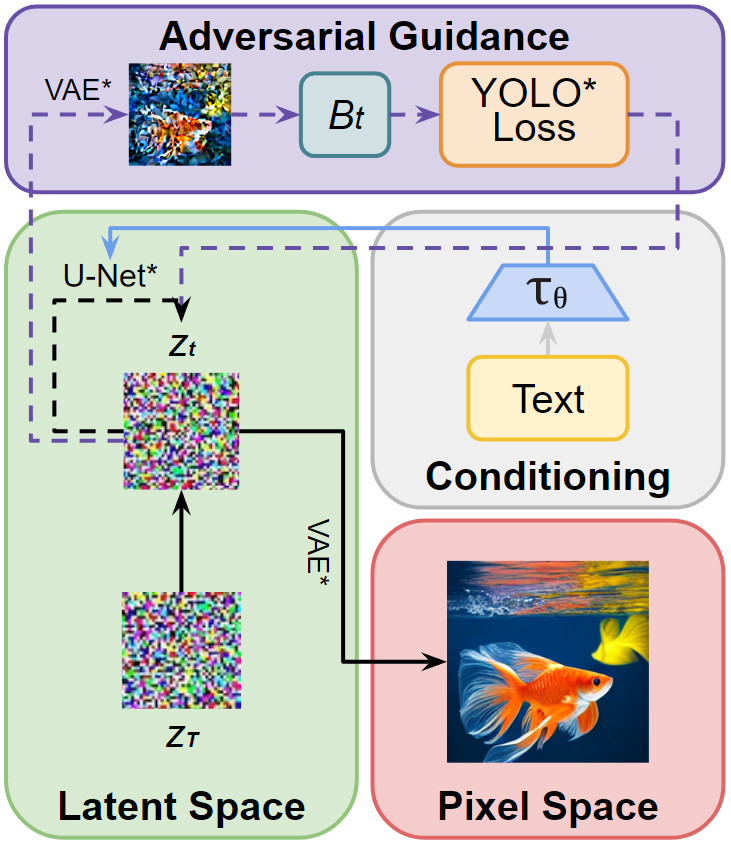
\includegraphics[width=0.45\linewidth, trim={0 0 0 0}, clip]{figures/sd_my_adv_common.png}
}
\caption{Stable Diffusion: original and modified pipelines.}
\label{sd_my}
\end{figure}

Figure~\ref{sd_my-a} depicts the original SD pipeline that was already introduced in Figure~\ref{sd}, albeit in a simplified form with the insides of U-Net hidden.
The sampling cycle that goes on for $T$ iterations is indicated by the gray dashed line: the U-Net model, taking into account the conditioning, predicts noise that should be removed from the latents at each step. 
After the cycle is completed, we leave the latent space for the pixel space with the help of VAE's decoder $\mathcal{D}$.

Figure~\ref{sd_my-b} introduces changes to this process.
Overall, the sampling pipeline stays the same, but we add a correction to our update direction in the form of adversarial detection guidance. 
That is, during the sampling process, we want to guide our latent not only towards generating a specific image according to our prompt conditioning, but also make it adversarial. 
Let us recall the guidance formula in general: 
$$\hat\epsilon_t = (1+s)\epsilon_\theta(z_t;t,y) - s\epsilon_\theta(z_t;t,\emptyset) + v\sigma_t\nabla_{z_t}g(z_t; t, y)$$

In order to define adversarial guidance, we have to understand what the energy function $g$ looks like in this case.
In essence, the energy function $g$ is some kind of adversarial detection loss; more formally, 
$$g(z_t; t, y) = s^{adv}_t \cdot \text{adv\_loss}(z_t, \mathcal{D}, \text{YOLO}, B_t)$$

where:

\begin{itemize}
    \item $s^{adv}_t$ is the adversarial guidance coefficient at step $t$. 
    It makes sense to change the intensity of adversarial guidance through the sampling process, so the entire set of adversarial guidance coefficient, $S^{adv} = \{s^{adv}_t\}^T_1$, is an important hyperparameter that will be later referred to as adversarial guidance scheduler;
    \item $z_t$ is intermediate latent that can be decoded into the corresponding intermediate noisy image $\Tilde{x_t}$ in the pixel space with VAE decoder: $\Tilde{x_t} = \mathcal{D}(z_t)$; 
    \item YOLO is our object detection model that is the key to obtaining the adversarial guidance; 
    \item $B_t = \{X_t, L_t\}$ is a batch of object detection images consisting of images $X_t$ and their labels $L_t$; 
    \item adv\_loss is our current method to extract the component of the real YOLO loss that is relevant to the task. 
    In our case, since we are working on evasion attacks, it will be the objectiveness score; in the general case, it can be any other meaningful part of the YOLO output, such as, for instance, the probabilities of predicted classes or bboxes.
\end{itemize}

Since $B_t$ mostly depends on the chosen pipeline type, further explanations of the formula will be introduced in the appropriate sections below.

Overall, the main idea is to alter the update direction of the conditioned update to arrive at an adversarial sample, much like classifier guidance from~\cite{dhariwal2021diffusion}.

\subsection{Adversarial Guidance Pipelines}

We have tried two techniques for calculating YOLO loss based on different approaches to obtaining data $B_t$ and applying $x_t$ to this data.
The pipelines are called 2D and 3D.
In the first pipeline, we use images from an existing labeled dataset with people, Inria Person~\cite{inria}.
$x_t$ are attached to the people from batch $B_t$ as patches.
With 3D pipeline, the background dataset~\cite{zh_3d} does not contain people; instead, human figures are dressed in clothes with tiled generations and rendered with certain augmentations.

\begin{figure}[htp]
\subfloat[2D]{
  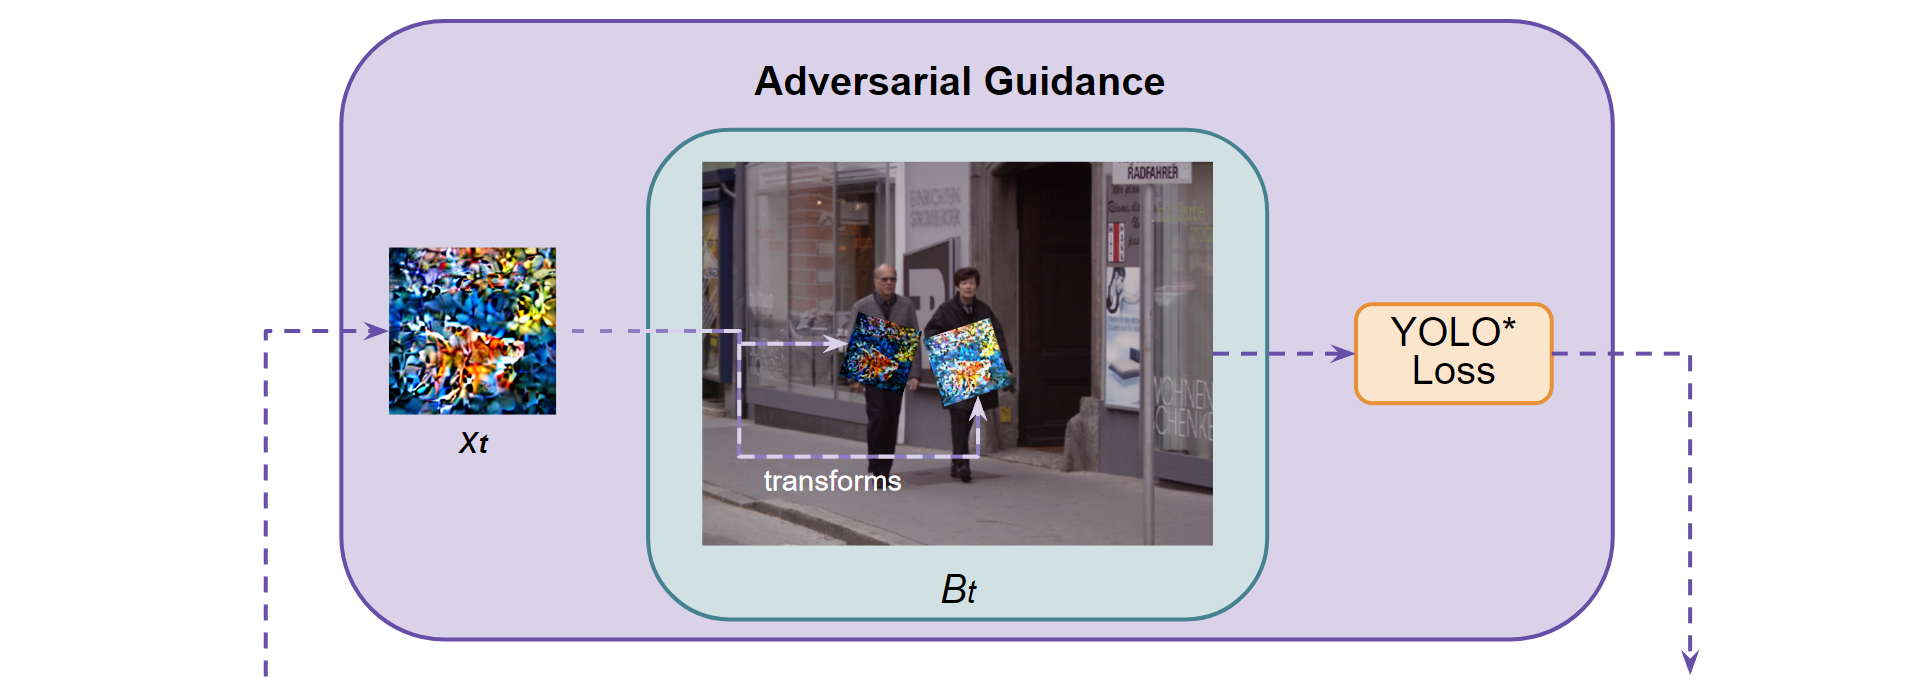
\includegraphics[clip, width=\columnwidth]{figures/sd_adv_2d.png}\label{ad_guid_a}
}\hfill
\subfloat[3D]{
  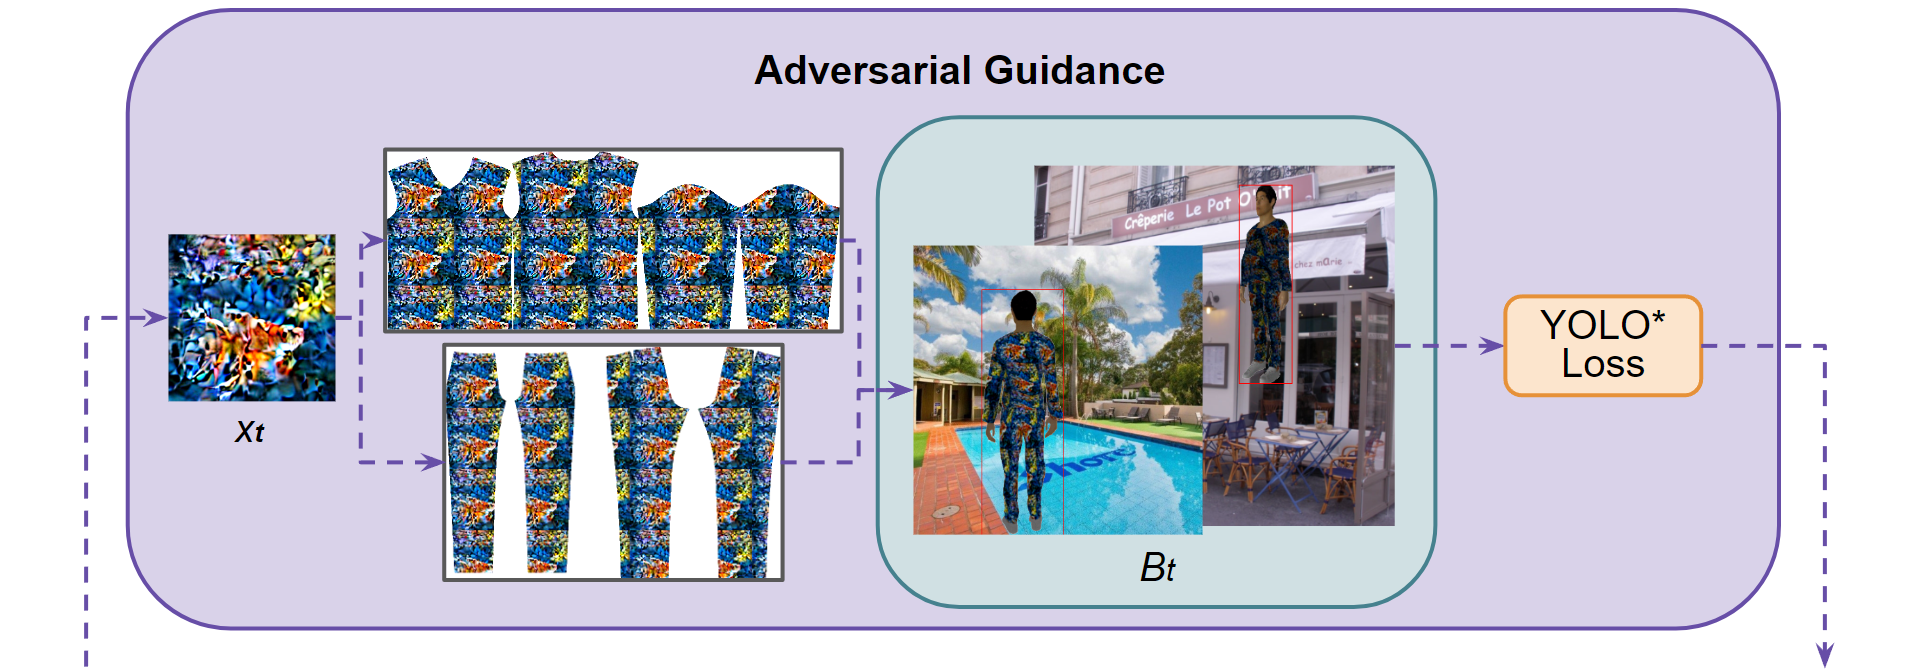
\includegraphics[clip, width=\columnwidth]{figures/sd_adv_3d.png}\label{ad_guid_b}
}
\caption{Adversarial Guidance Pipelines}
\end{figure}

The pipelines are shown on Figures~\ref{ad_guid_a} and~\ref{ad_guid_b}.


\paragraph{2D} In the case of 2D pipeline, intermediate partially denoised images $x_t$ are attached to all people from every image $X_{tm}$ in batch $B_t = \{(X_{tm}, L_{tm})\}_1^M$ consisting of $M$ images.
We are trying to lower the highest confidence of relevant bboxes, so the energy function in this case is:
$$g(z_t; t, y) = s^{adv}_t \sum_{m=1}^M \max \text{\LARGE [} \text{yolo\_loss}\text{\large (}\Tilde{X}_{tm}, L_{tm}\text{\large )}_{\text{obj}} \text{\LARGE ]}$$

where $\Tilde{X}_{tm}$ is $X_{tm}$ with attached augmentations of $x_t$, yolo\_loss is the regular loss for the YOLO, and $_{\text{obj}}$ signifies that we only look at the objectiveness (confidence) scores of the predictions, since we are performing an evasion attack and want to not be detected. 

In this case, augmentations consist of the standard simple transformations like adjustments of brightness, angle, contrast, and adding random noise, and also applying Thin plate splines (TPS, see Section~\ref{sec:tps} below).
All of the applied transformations are differentiable. 

\paragraph{3D} 
In the case of 3D adversarial guidance pipeline, we first tile our generated texture $x_t$ to cover a 3D model's clothes $C_t$.
Afterwards, using a 3D rendering module of Python, we render a 3D model that we have prepared in advance with help of~\cite{zh_3d}.
The models are rendered on random backgrounds from the dataset.
We also sample light and camera angles to ensure the effectiveness of our attack in the real world. 
This, as well as the 3D TPS, TopoProj (see Section~\ref{sec:tps}),  and shifting of the initial position of $x_t$ on $C_t$, are our augmentations.

The energy function is essentially the same as in the 2D case, albeit it is important to note that in this case, labels $L_{tm}$ are not provided in the dataset, but rather calculated according to the current sampling and rendering strategy that changes over time, and images $X_{tm}$ contain rendered figures as shown on Figure~\ref{ad_guid_b}.

\subsection{TPS and TopoProj}\label{sec:tps}

One of the most important augmentations we use in this task is TPS. 

 TODO 

Another important technique that was introduced in~\cite{zh_3d} is TopoProj.

 TODO 

% \subsection{Obtaining Latents}

% The simplest way to obtain the latent corresponding to an input image is to take the encoder part of the pretrained diffusion model, $\mathcal{E}$ from Figure~\ref{sd}.
% Otherwise, it is also possible to use the paper called ``Null-text Inversion for Editing Real Images using Guided Diffusion Models'' for obtaining the latent.
% In this paper, the authors introduce a method to improve the basic DDIM inversion so that it works better with classier-free guidance that is also used in our main pipeline.


\section{Appearance Restoration}

As we have stated previously, we want our adversarial evasion clothes to be controllable: that is, we are able to obtain not just a random adversarial pattern, but rather be able to make it closer to something we want to see specifically.
Let us say we have a simple non-adversarial sampling trajectory of our SD $\hat{z}_T\ldots\hat{z}_0$ that leads us to our desired image $\hat{x} = \mathcal{D}(\hat{z}_0)$.
Now we are trying to generate $x$, an adversarial texture for clothes that at the same time is close to our original $\hat{x}$.
Firstly, we make a step according to our U-Net prediction; secondly, this direction is modified with adversarial guidance. 
The trajectory, however, can change significantly compared to the original one, so $x$ can be very different from $\hat{x}$ if the adversarial scheduler $S^{adv}$ consisted of large coefficients.

So, we have to propose a method to preserve the original appearance, even maybe at the cost of adversarial effectiveness. 
In order to do that, we insert additional appearance restoration guidances that push our generation in the direction of the original sampling trajectory.
We have tried guidances dictated by two different losses that we will introduce in this section.

\subsection{Appearance Constraint Loss}

Since the attention maps of U-Net contain information about the position and the form of objects and the activations from appropriate layers store the appearance of the objects, it is possible to manipulate several properties of the objects using the representations stored in the U-Net layers.
% TODO 

Following~\cite{aibek}, let us define the appearance of objects in terms of the information stored in U-Net.
Let us denote an intermediate attention map from layer $n$ on timestamp $t$ as $\mathcal{A}_{t,n} \in \mathbb{R}^{P \times H_n\times W_n}$, where $P$ is the length of the prompt (one word is one channel starting with position 1; empty tokens are added at the end until we reached the intended length $P$).
Similarly, activation (features) will be denoted as $\mathcal{F}_{t,n}\in \mathbb{R}^{F_n\times H_n\times W_n}$.

According to~\cite{att_replace_silver_robots}, attention maps store information about the shape and the position of the objects from their corresponding channels.
That is, by looking at the attention maps $\mathcal{A}_{t,:}$ at timestamp $t$, we can see the shape of all objects; if we want to see the shape of $p$-th object from layer $n$, we should look at $\mathcal{A}_{t,n,p}$.
The bigger the value in the corresponding channel, the more related the pixels are to this word.
Omitting timestamps and layering indexing, the following formula can be used to calculate the shape of object $p$:
$$\text{shape}(p) = \mathcal{A}_p$$

In practice, attention maps $\mathcal{A}$ are thresholded to account for background noise. 
It is possible to change the shape of object by guiding these maps towards those of another generation or provided by the user, but in our case, we are interested in the entire appearance of objects that can be expressed as:
$$\text{appearance}(p) = \dfrac{\sum_{h,w}\text{shape}(p)\odot \mathcal{F}}{\sum_{h,w}\text{shape}(p)}$$

This formula makes sense because $\text{shape}(p)$ creates a mask that denotes the form of object $p$ and activation maps represent local appearance.

To use appearance constraint as guidance, we need to define the energy function $g$.
As we have mentioned in the introduction part of this section, we already have our original generation $\hat{x}$ and latent trajectory that leads to it. 
That is, we can run the SD to obtain this trajectory $\hat{z}_T\ldots\hat{z}_0$.
While running this process, we can store all the intermediate U-Net attention maps and activations to be able to reconstruct the original $\widehat{\text{appearance}_t(p)}$ for object $p$ on timestamp $t$ of this original run.
With this, we can use attention constraint guidance as the gradient obtained from the l1-loss between the original appearance and the current appearance of object $p$:
$$g(t, p) = s^{ap}\cdot \text{l1-loss}(\text{appearance}_t(p), \widehat{\text{appearance}_t(p)})$$

where $s^{ap}$ is the corresponding guidance coefficient.

In our case, we want the entire generation to be close to the original, so we add the guidance to all words in the prompt as $\sum_{p\in P} g(t,p)$.

\subsection{Attention Constraint Loss}

Even though the method helps to fix the appearance of the generation, fixing all words is a prompt has little physical meaning.
For example, for a prompt ``a beautiful goldfish swimming through the ocean'', it is easy to imagine what objects like ``goldfish'' and ``ocean'' do look like, but it fixing parts of prompt like ``a''/``through'' or ``swimming'' is unjustified.
This is why we suggest to only fix self attention maps that restrict the affinities between the features. 
Self-attention maps control the layout of the image in the lower layers and capture details on higher, so guiding them will guide the entire image to the original $\hat{x}$.

Similarly to appearance constrain loss, we have to run the original trajectory $\hat{z}_T\ldots\hat{z}_0$ and store all self-attention maps $\hat{\mathcal{A}}^{self}_t$ on all timestamps $t$.

The guidance can be defined as l1-loss for the original and newly generated self-attention maps:
$$g(t) = s^{at}\cdot \text{l1-loss}(\mathcal{A}^{self}_t, \hat{\mathcal{A}}^{self}_t)$$

TODO for this and previous subsections: illustrations (?)

\section{Final Algorithm for 3D Pipeline}

\begin{figure}[ht!]
\centering
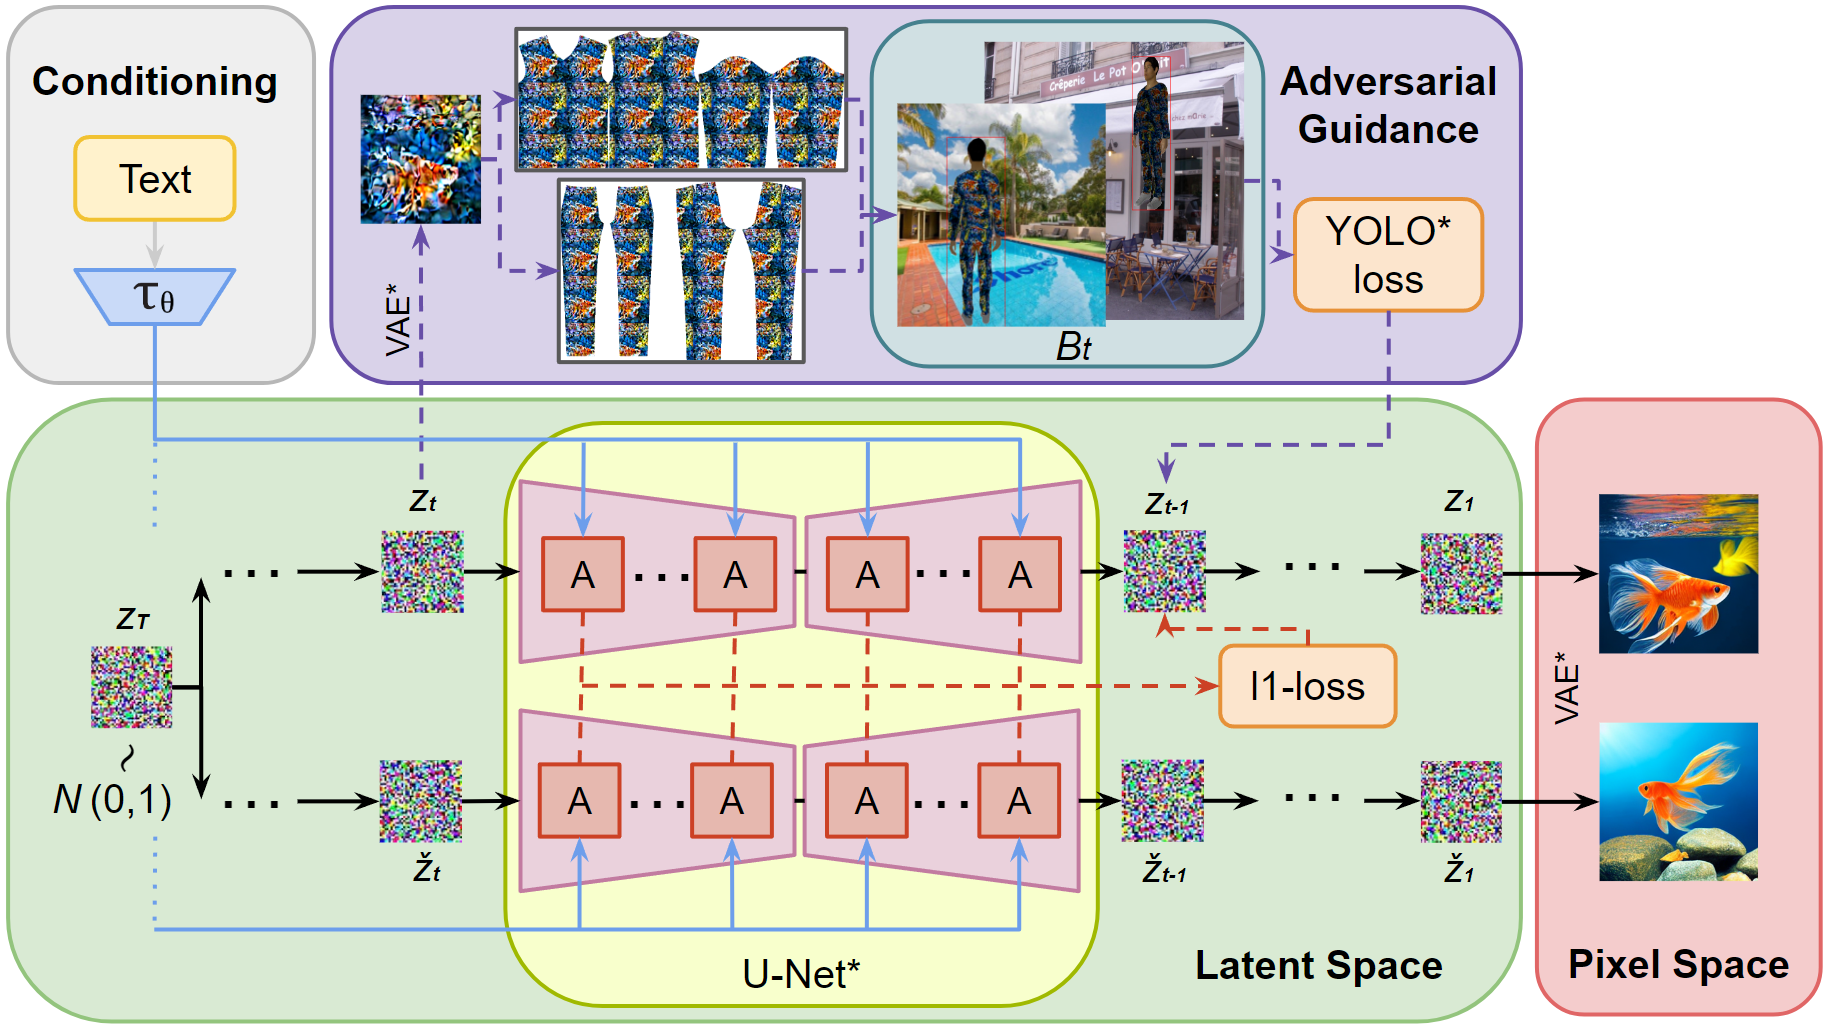
\includegraphics[width=150mm]{figures/sd_adv_fix_3d.png}
\caption{Final pipeline with both adversarial and fixation guidances.}
\label{sd_3d_adv_fix}
\end{figure}

In our case, for the $g$ energy function, we chose YOLO loss.
Again, the physical explanation of this guidance is that we are trying to maximize YOLO loss for the predicted people, so that ultimately our patch helps in avoiding detection by this YOLO:
$$\nabla_{z_t}g(z_t; t, y) = s^{adv}_t \sum_{m=1}^M \nabla_{z_t}\max \text{\LARGE [} \text{yolo\_loss}\text{\large (}\Tilde{X}_{tm}, L_{tm}\text{\large )}_{\text{obj}} \text{\LARGE ]}$$

So, compared to the standard SD sampling, we allow latent $z_t$ to accumulate gradients and add this gradient to our update $\hat\epsilon_\theta$.
In this section, we will provide the adversarial algorithm for our pipeline that is fully shown in Figure~\ref{sd_3d_adv_fix} on the example of the combination of two guidances: adversarial and attention constraint.


\renewcommand{\algorithmicrequire}{\textbf{Inputs:}\unskip}
\renewcommand{\algorithmicensure}{\textbf{Output:}\unskip}
\renewcommand{\algorithmiccomment}[1]{\textcolor{gray}{{\scriptsize$\triangleright$}\,#1}}


\begin{algorithm}
  \caption{Sample adversarial $x$ based on non-adversarial $\hat{x}$}
  \label{alg1}
  \small
  \begin{algorithmic}
    \REQUIRE Prompt $\mathcal{P}$, number of SD steps $T$, adversarial scheduler $S^{adv}$, attention constraint coefficient $s^{at}$, adversarial dataset $DS$

    \STATE $z_T \sim \mathcal{N}(0, 1)$\hspace{2.38cm}
    \COMMENT{initial noisy latent}
    
    \STATE $P_{emb} \gets \tau(\mathcal{P})$\hspace{2.5cm}
    \COMMENT{CLIP prompt encoding}

    \STATE {$\text{self\_att\_maps} \gets []$} 
    \FOR{$t \leftarrow T$ to $1$}
        \STATE {$\text{self\_att\_maps.register(U-Net.self\_attention)}$}\quad
	\COMMENT {saving attention maps for non-adv sampling}
        \STATE $\epsilon \gets \text{U-Net}(z_t, P_{emb})$
        \STATE $z_{t - 1} \gets \text{update}(z_t, \epsilon)$
    \ENDFOR

    \FOR{$t \leftarrow T$ to $1$}
        \STATE $\epsilon \gets \text{U-Net}(z_t, P_{emb})$
        \STATE $x_t \gets \mathcal{D}(z_t)$\hspace{2.32cm}
	\COMMENT{decoding latents into intermediate images}

	\STATE $X, L = DS\text{.next\hspace{0.05cm}}()$
        \STATE $\Tilde{X} \gets X.\text{attach}(x_t)$\hspace{1.3cm}
	\COMMENT{obtaining augmented image for YOLO}

        \STATE $\epsilon \gets \epsilon + S^{adv}_t\nabla_{z_t}\text{YOLO-loss}(\Tilde{X}, L)$\hspace{4.127cm}
	\COMMENT{adv guidance}

        \STATE $\epsilon \gets \epsilon + s^{at}\nabla_{z_t}\text{l1-loss(U-Net.self\_attention, self\_att\_maps[t])}$\quad
	\COMMENT {appearance guidance}

        \STATE $z_{t - 1} \gets \text{update}(z_t, \epsilon)$
    \ENDFOR

    \STATE $x \gets \mathcal{D}(z_0)$
    \ENSURE Adversarial $x$
  \end{algorithmic}
\end{algorithm}

The method is shown in algorithm~\ref{alg1} in pseudocode. 
Just as the usual SD pipeline, we start by generating the initial noisy latent $z_T$ (in case it was not provided by the user in the input data).
We also have to use our text encoder, typically CLIP, to create prompt embeddings $P_{emb}$.

After that, we run the first sampling that is non-adversarial.
We need to do this since we intend to save attention maps from all intermediate steps to be able to guide our adversarial trajectory in the direction of the original path.
So, during the first cycle, we save all needed information from U-Net, which, in case of attention constraint guidance, are self-attention maps only.
The cycle itself is standard for SD: we generate noise prediction $\epsilon$ with the U-Net model and then use it to update the current latent $z_t$. 
In the actual pipeline, we also use classifier-free guidance described in Section~\ref{sec:guidance} by running the U-Net model for two inputs simultaneously, but this part is omitted in the pseudocode for its irrelevance to this method as it is used for improving results in general rather than its adversarial effects.

After the initial self-attention maps are stored, we can start running the adversarial sampling.
Now, on each iteration of standard SD sampling, we perform the following additional operations after obtaining noise prediction $\epsilon$ on step $t$:

\begin{enumerate}
    \item Use our frozen VAE model (decoder $\mathcal{D}$ from Figure~\ref{sd}) to obtain $\hat x_t$;
    \item Transform this $\hat x_t$ into clothes $\hat c_t$ for our 3D model;
    \item Render human figures dressed into the clothes $\hat c_t$ into scenes from the background dataset while performing augmentations to ensure effectiveness in physical attacks to create images $\Tilde{X}$ for YOLO;
    \item Calculate the YOLO detection loss for the scenes with our augmented $\Tilde{X}$ and their labels $L$;
    \item Perform adversarial guidance: add gradient $\nabla_{z_t}$ from this loss to the noise prediction $\epsilon$ with coefficient $S^{adv}_t$;
    \item Calculate the l1-loss between the current self-attention maps of U-Net and those we have saved from the original run;
    \item Perform attention constraint guidance: add gradient of the loss in the previous step to the noise prediction $\epsilon$ with coefficient $s^{at}$.
\end{enumerate}

Each iteration of the cycle is finished with updating latent $z_t$ with obtained guided noise $\epsilon$.

After the sampling cycle is completed, we can obtain our final adversarial $x$ as the decoded final latent: $x = \mathcal{D}(z_0)$.

\section{Tiling}

So far, we have not discussed why our method is natural considering the fact that we simply tile generated pictures are not necessarily tileable.
However, the section with experiments will show examples of generated patches that can be tiles almost seamlessly.
In this section, we describe our original method to achieve this effect without any additional guidance.

\paragraph{Prompt Modification}

\begin{figure}[htp]
\subfloat[Two levels of prompt extensions: the second level (the last row) contains patterns that can be tiled.]{
  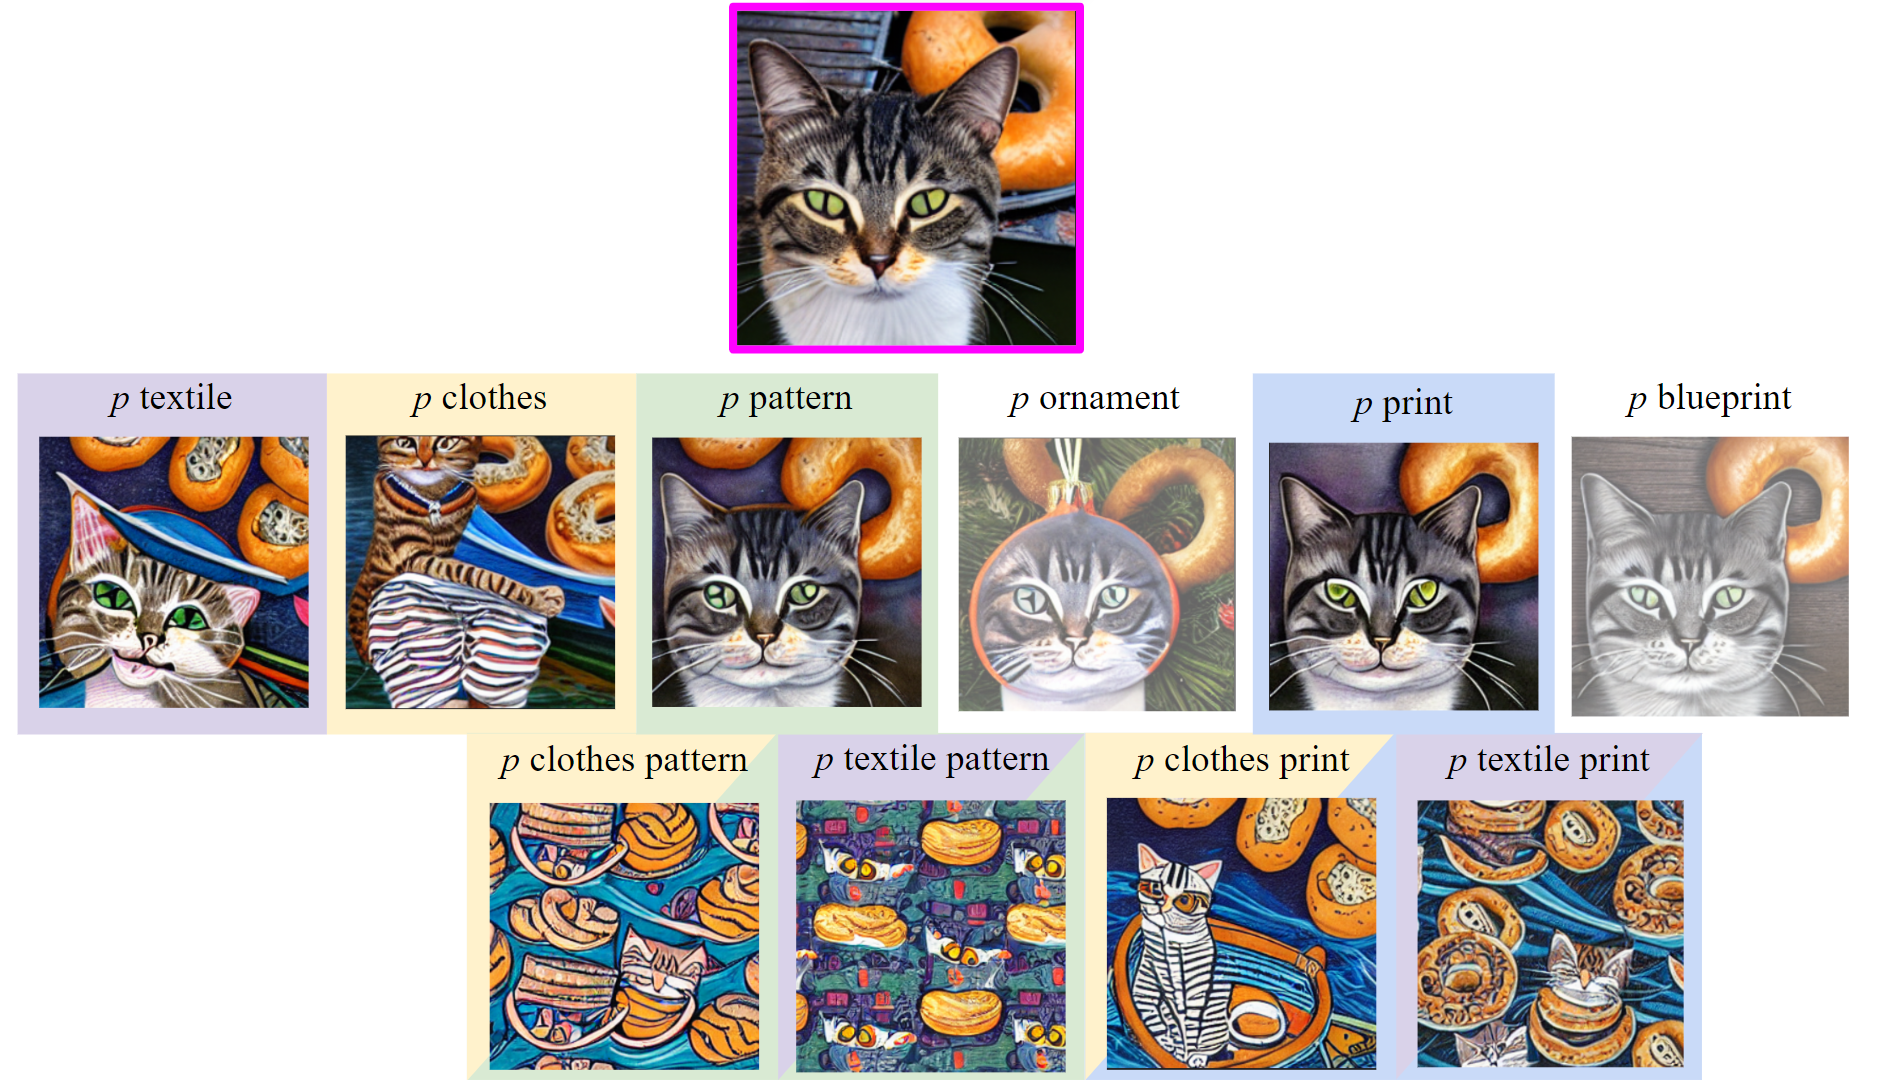
\includegraphics[clip, width=\columnwidth]{figures/tiling1.png}\label{tiling_a}
}\hfill
\subfloat[Stacking specific lines increases the effect.]{
  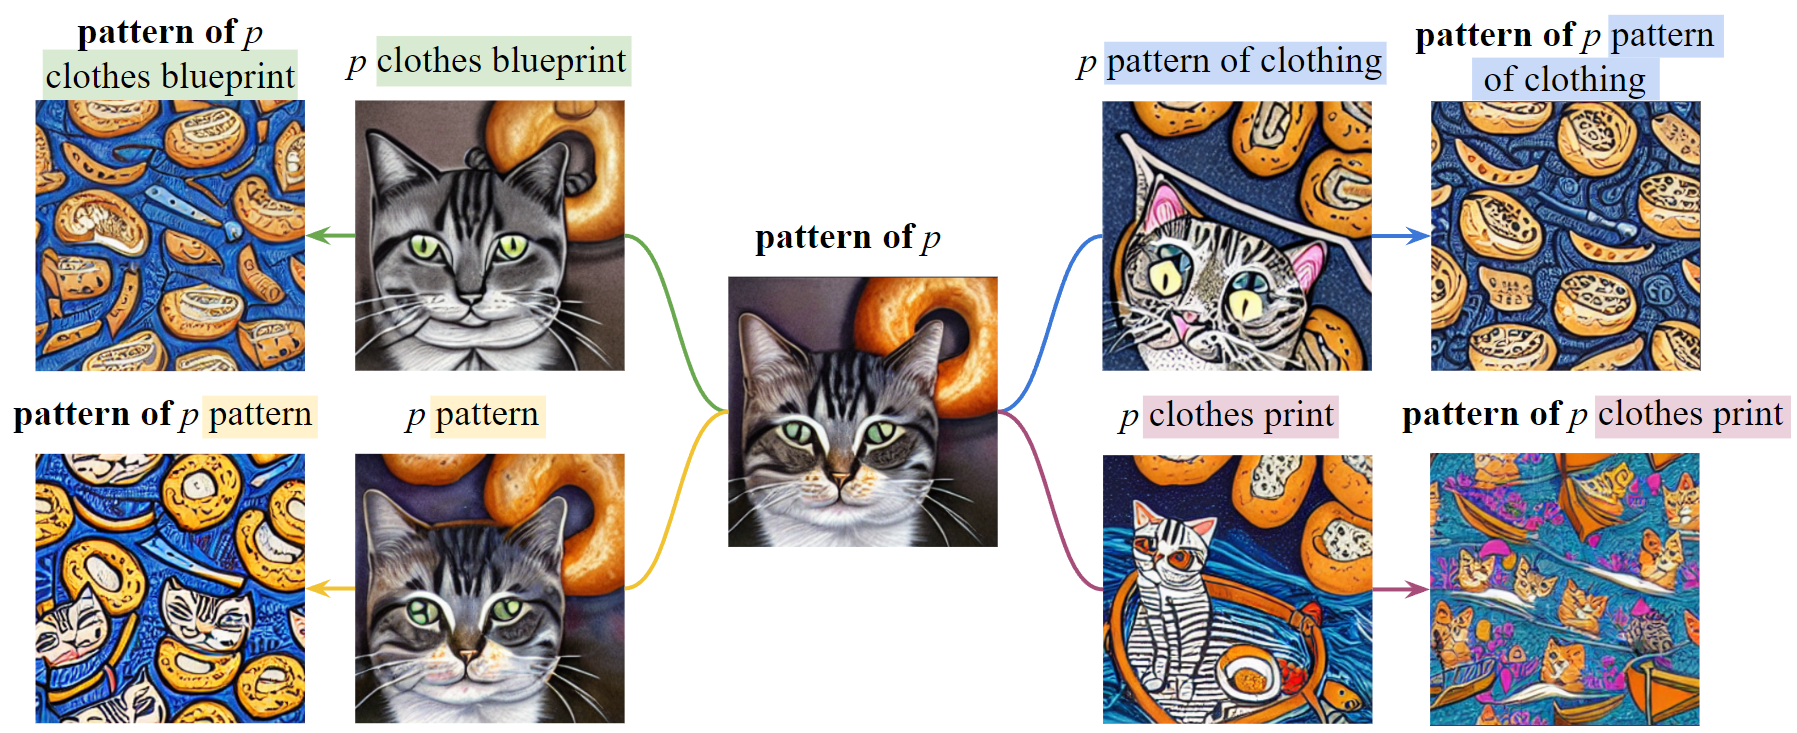
\includegraphics[clip, width=\columnwidth]{figures/tiling2.png}\label{tiling_b}
}
\caption{Prompt modifications for prompt $p$ ``A cat on a boat with a bagel'' (the highest image in a dark pink box).}
\end{figure}

The SD model is trained on a large dataset LAION~\cite{laion} that consists of roughly 5 billion images, so the model manages to learn many nuances of the text-image relationship, which can be used by modifying the input prompt.
It turns out that it is possible to modify the prompts to make the SD produce textures that can be tiled almost seamlessly.

Figure~\ref{tiling_a} shows several such examples.
In the upper row, we have the original generation for a random prompt --- ``A cat on a boat with a bagel''.
In the second row, we extend this prompt by adding one word that is related to our task, but do not obtain tileable textures just yet. 
In the last row, we show some of the combinations of the prompt extensions above. 
Three of them, ``\textit{p} clothes pattern'', ``\textit{p} textile pattern'', and ``\textit{p} textile print'' achieve the needed effect: if we put any of these generations side by side with itself, the final pattern will be smooth.
However, only a limited number of such combination works, and, for example, combining words ``\textit{p} textile'' and ``\textit{p} pattern'' with ``\textit{p} ornament'', and ``\textit{p} blueprint'' yield no needed results, and the generated patterns for these combinations in essence look like ``\textit{p} clothes print'' in the last row, which can not be tiled.

Interestingly, stacking these lines, we can enhance the effect, turning generations even for the non-effective first level extensions tileable.
Examples of this are shown on Figure~\ref{tiling_b}.
This set of examples for the same prompt demonstrates the effectiveness of the prompt command ``pattern of \textit{p}''.
By itself, as we can see from the image in the middle, the word does not make our random prompt generation continuous.
The same goes for four other prompt extensions that are connected to the image in the middle: ``\textit{p} clothes blueprint'' (green), ``\textit{p} pattern'' (yellow), ``\textit{p} pattern of clothing'' (blue), and ``\textit{p} clothes print'' (purple).
However, if we combine the original ``pattern of \textit{p}'' with any of the four aforementioned extensions, we will obtain the outer set of four images that can be put side by side to create continuous patterns.

\paragraph{Tiling vs Adversarial Effect}
% TODO theres no conflict

\begin{figure}[htp]
\centering
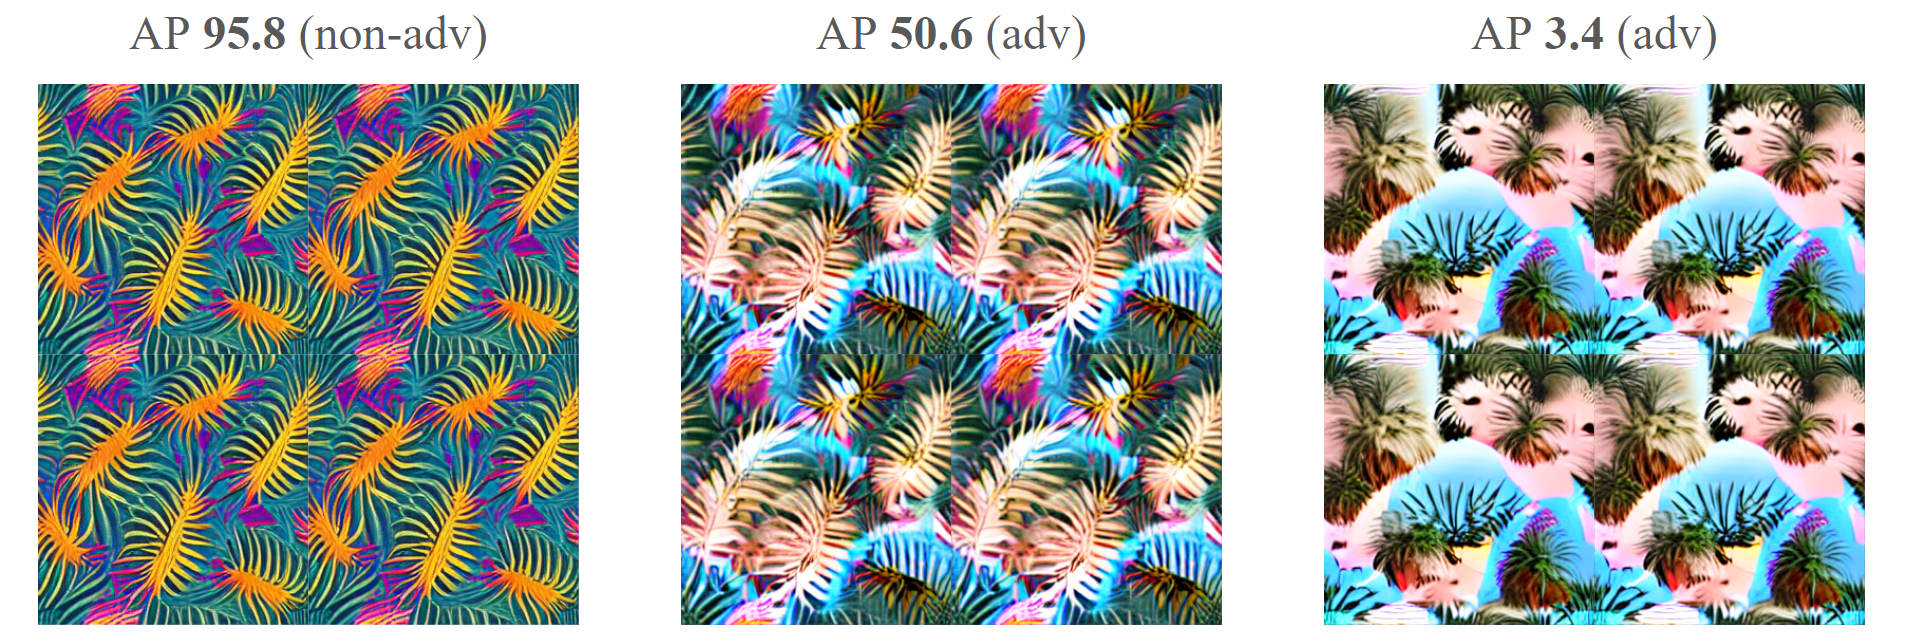
\includegraphics[width=150mm]{figures/adv_vs_tiling.png}
\caption{The generations are still tileable as we apply stronger adversarial guidances.}
\label{tiling_vs_adv}
\end{figure}

Importantly, this effect does not diminish as we add adversarial guidance to our generation.
To demonstrate this, we show three generations for the same prompt, ``palm clothes pattern'', in Figure~\ref{tiling_vs_adv}, which also shows what we mean by ``tileable'' images.
Here, in the left part, we have the original non-adversarial generation for the prompt repeated 4 times to demonstrate that the tiling has indeed almost negligible seams on the joints.

The next two parts of the figure show examples of adversarial and appearance-restorated generation for the same prompt. 
The middle one has little adversarial effect due to the weak adversarial scheduler and strong attention and appearance constraining guidance coefficients, so the average precision (AP) is rather high.
At the same time, the rightmost part shows an example of a highly adversarial image with little resemblance to the original generation. 

Yet all of these three generations can be tiled very well, and a stronger adversarial scheduler does not mitigate the tiling prompt extension, which, in this case, is ``clothes pattern''.

\paragraph{Problems}

\begin{figure}[htp]
\centering
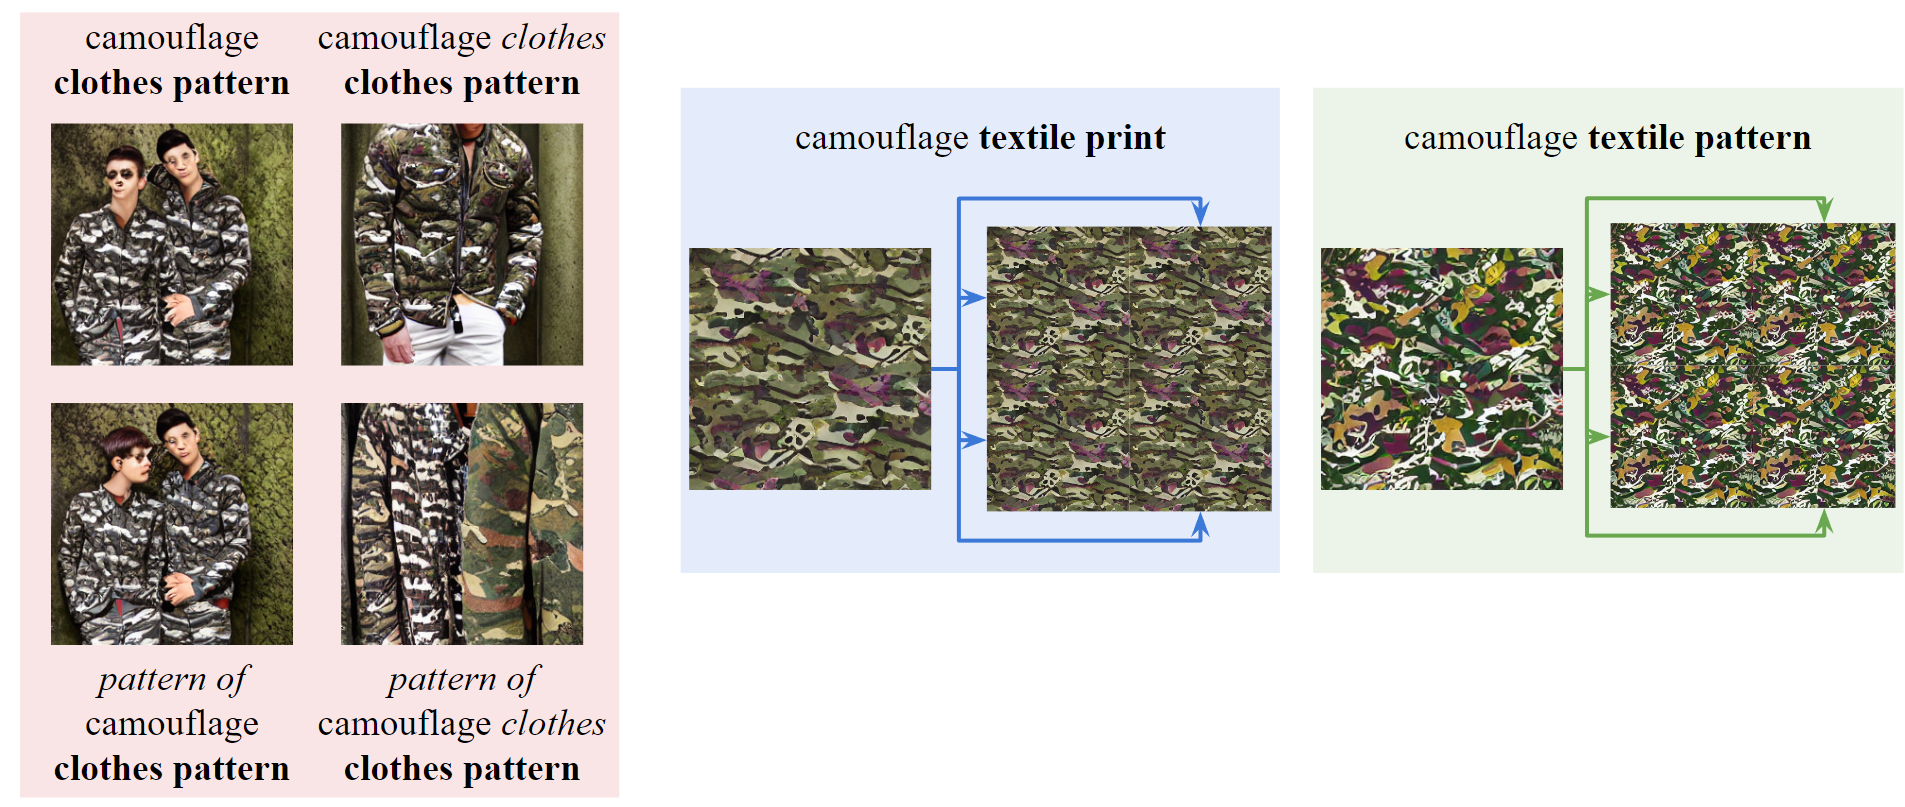
\includegraphics[width=150mm]{figures/clothes_pattern_fails.png}
\caption{``clothes pattern'' extension fails.}
\label{clothes_pattern_fails}
\end{figure}

The obvious problem of this approach is that there is nothing that guarantees that the chosen prompt extension will work as intended, creating a continuous pattern.
For example, the ``clothes pattern'' extension fails on the ``camouflage'' prompt, as shown in the upper-left image of the red part of  Figure~\ref{clothes_pattern_fails}.
This can be explained by the fact that words like ``camouflage'' and ``clothes'' often go together, so the SD model has learned some additional dependencies and creates specific generations like the one we observe.
Adding another ``clothes'' or enhancing the tiling effect with an additional ``pattern of'', as suggested in the example of Figure~\ref{tiling_b}, does not solve the problem.

Even though this particular problem can be solved by choosing another prompt extension like ``textile print'' or ``textile pattern'', as demonstrated in the blue and green parts of Figure~\ref{clothes_pattern_fails}, there is no guarantee that these other extension work for all possible prompts.

\paragraph{TV-loss}
TODO?

\section{Datasets}

In this section, we briefly describe the datasets that have been used during the research and our methods to add clothes to the generated data.

\paragraph{Inria Person}

TODO

\paragraph{Background}

TODO

\section{Evaluation}

In this section, we will briefly introduce the metrics that we are most likely to use for the evasion task.

\paragraph{IoU threshold}
Whether a box predicted by a detector is considered a valid object is decided based on the intersection over union (IoU) score.
In case if there are many overlapping boxes on a test image like in the Inria Dataset that is often used for evaluation, a relatively high IoU threshold of 0.5 is usually chosen.
However, a high threshold value may lead to overestimation of the effectiveness of the attack, so we intend to study different values.

\paragraph{AP} 
TODO 

\paragraph{ASR}
We define Attack Success Rate (ASR) as the ratio between the incorrectly predicted test images to the total number of test images.
An object is considered as correctly identified if the objectiveness score for it is higher than 0,5.
% TODO 

\paragraph{Naturalness}
~\cite{dog_patch_clothes} suggested using subjective evaluation to get a naturalness score of a patch.
For this evaluation, a number of participants is invited to estimate how natural the clothes in question look.
A naturalness evaluation is not difficult to perform since the number of participants should not necessarily be very high---in~\cite{dog_patch_clothes}, it was 24.
% TODO water

TODO describe problems with metrics

\section{Experiments}

In this section, we present the results of the method in different scenarios.
% TODO more about what we analyse 

\subsection{2D Pipeline}

\begin{figure}[htp]
\centering
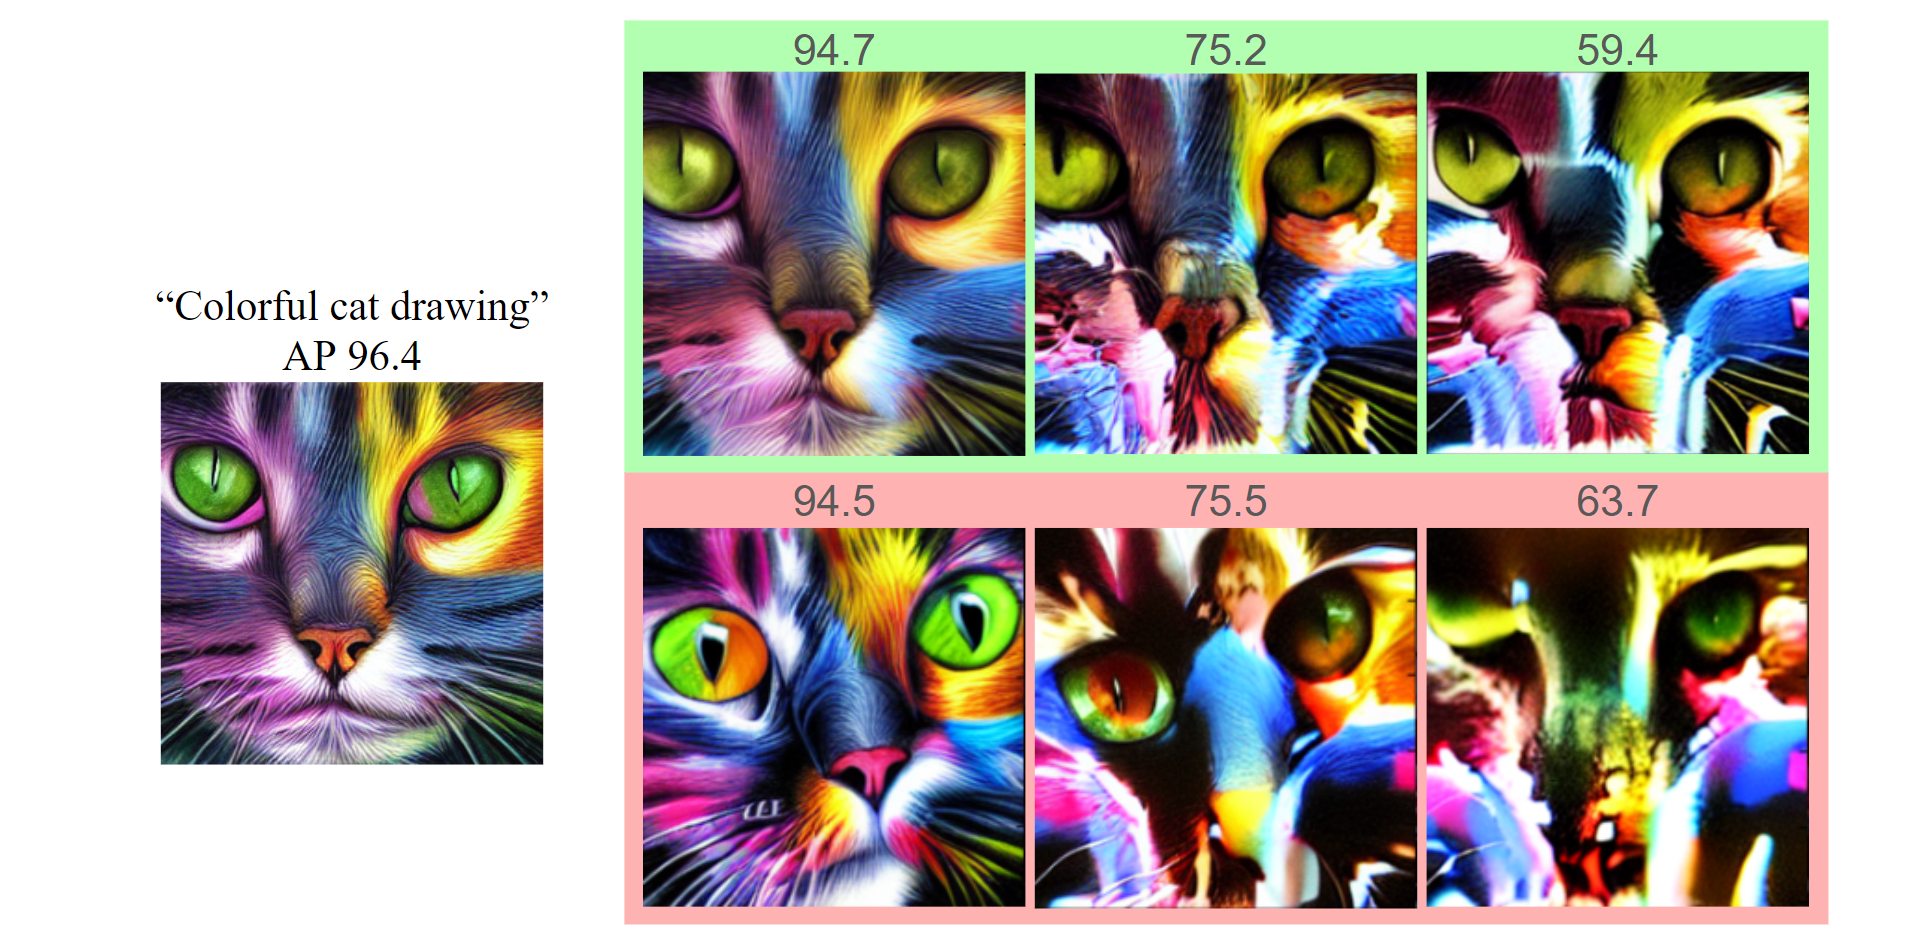
\includegraphics[width=150mm]{figures/2d_res.png}
\caption{Experimental results for 2D pipeline, prompt ``colorful cat drawing''. Only adversarial guidance.}
\label{2d_res}
\end{figure}

Figure~\ref{2d_res} presents results obtained with the 2D pipeline for prompt ``colorful cat drawing'' for the original SD generation on the left and 6 adversarial generations with different schedulers on the right.

The upper green row shows relatively good results: the AP decreases as we trade naturalness of the picture for its effectiveness.
The lower red row is significantly worse: we stray far away from our original generation on the left while achieving similar APs; moreover, the last two generations do not even appear natural.
As a reminder, we also reiterate the reason why we want our adversarial generation to be close to the original image: we want to be able to control our final result, so, instead of just obtaining any image from the ``colorful cat drawing'' space, we want something close to provided image.

The first image in the lower world looks realistic, but has a high AP and is very far away from the original image.
The reason behind this is that the scheduler that was used to create this generation had very high adversarial coefficients in the beginning and low by the end of the generations.
Basically, we just started from a different noise and arrived at another natural image that just happened to be more adversarial.
While optimizing latent as another part of the pipeline is promising in terms of adversarial effectiveness, we would have lost any control as soon as we switched to this method.

\begin{figure}[htp]
\centering
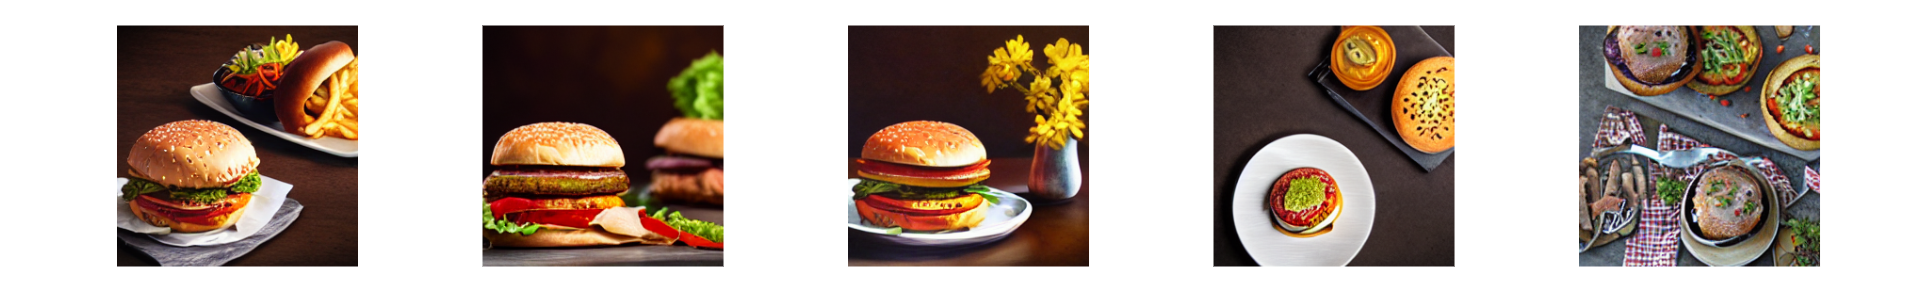
\includegraphics[width=150mm]{figures/hamburger.png}
\caption{``A hamburger on a table'', SD. Different number of steps between 30 and 512.}
\label{hamburger}
\end{figure}

Moreover, more often than not, a random noise that leads to higher adversarial effects also has absolutely unnatural non-adversarial generations.
For example, for the ``a hamburger on a table'' prompt, SD generates very different results depending on the number of steps, as demonstrated in Figure~\ref{hamburger}.
The same generally holds true for all prompts.
It turns out that we can achieve higher adversarial effects if we guide the last generation; however, as we can see, this additional effectiveness comes at the cost of naturalness as well, so we do not look for the best starting latent and rather focus on controlling the generation process to produce something close to the original image.
This also reinforces the theory that appearance constraint guidance is very important for our method.

The major problem of this approach is the fact that the APs are undeniably high, while the naturalness fades away rather swiftly; even more importantly, we are unable to achieve lower APs with this method, and higher coefficients in adversarial schedulers only lead to complete vanishing of naturalness and no decrease in adversarial effectiveness, like in the last generation with AP 63,7.

This is the initial pipeline we used, and it turned out to be so much less effective than the 3D pipeline that examples of the results are only presented in this subsection; the rest of this section is dedicated to the 3D pipeline.

\subsection{Adversarial Guidance}

\begin{figure}[htp]
\centering
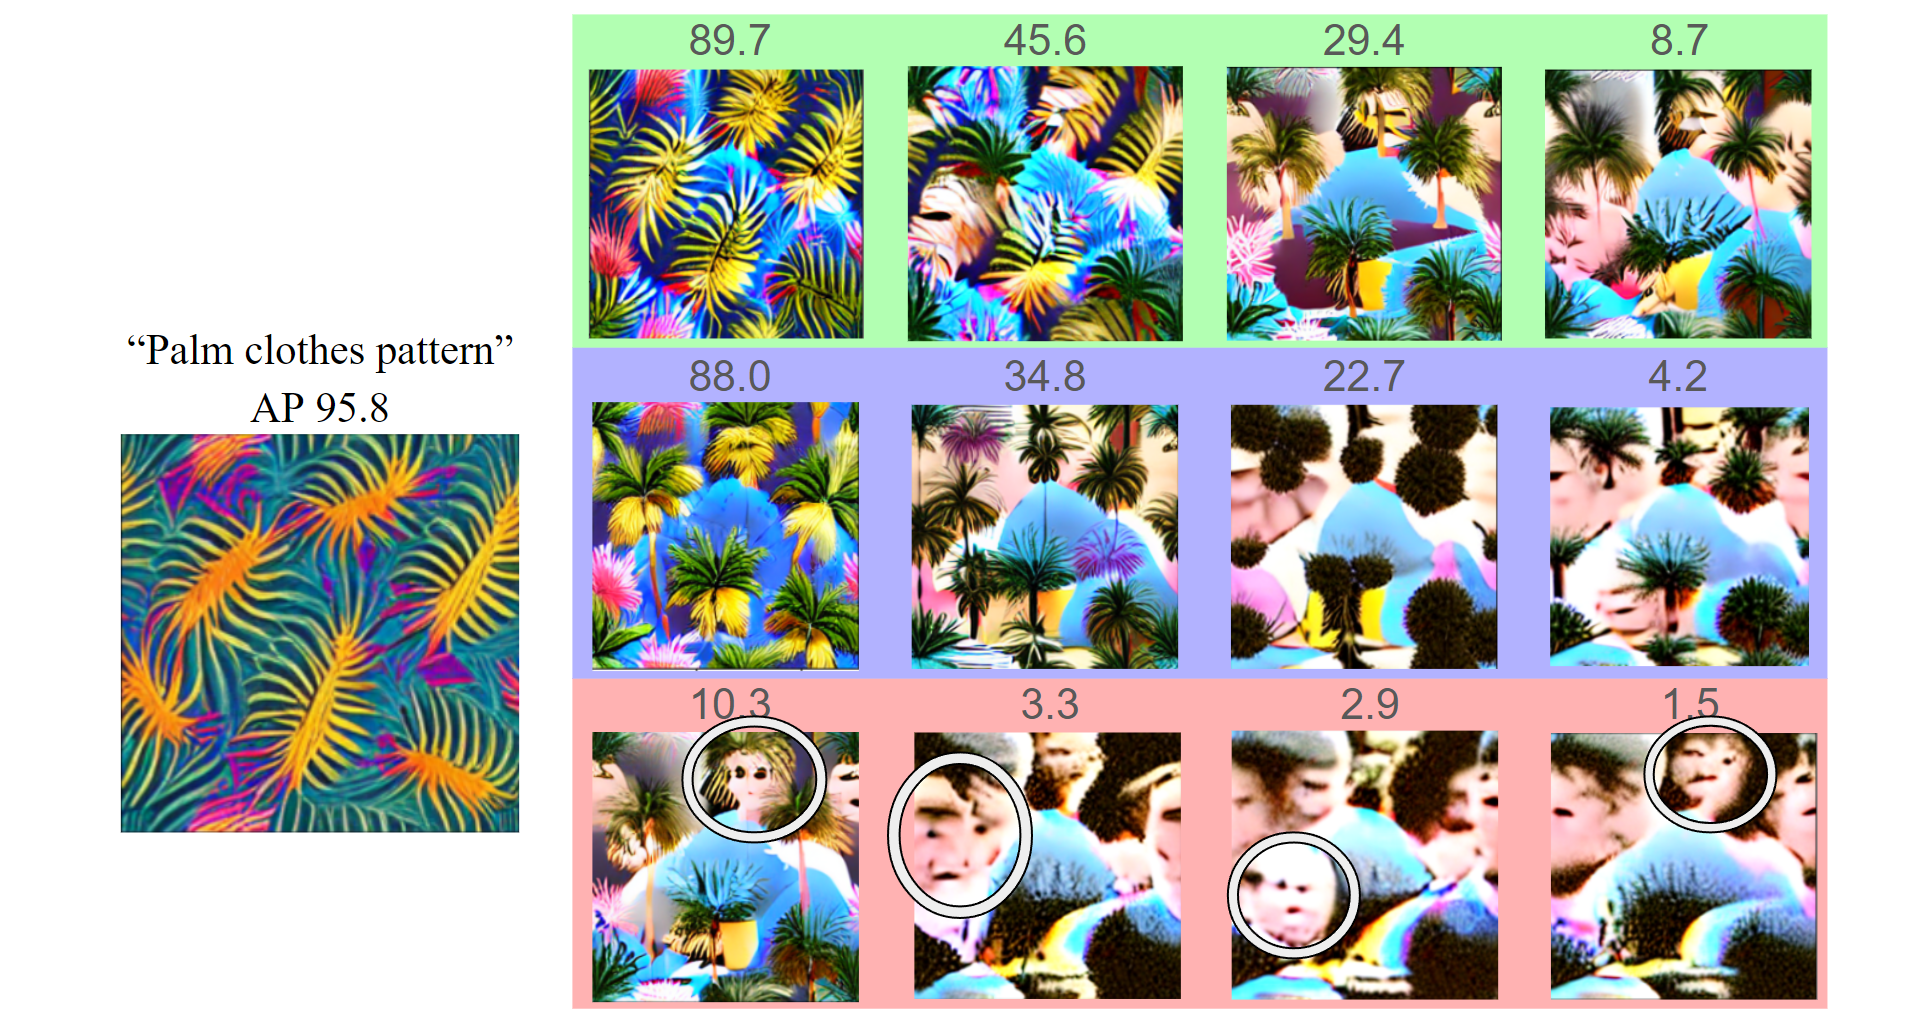
\includegraphics[width=150mm]{figures/3d_res_wo_fix.png}
\caption{Experimental results for the 3D pipeline, prompt ``palm clothes pattern''. Only adversarial guidance.}
\label{3d_wo_fix}
\end{figure}

After switching to the 3D pipeline, we immediately achieve much lower APs, as shown in Figure~\ref{3d_wo_fix} on the example of the ``palm clothes pattern'' prompt adversarial generations for 12 different schedulers. 

The generations on the upper green row are good and follow our expectations: as we apply stronger adversarial guidance coefficients, we go further away from the original non-adversarial generation on the right but also avoid detection better.
Even though the last two images in this row do not resemble the original generation, we at least still observe ``palms'' in the resulting patches. 

For the second blue row, while the adversarial effects are similar to the upper row, the generations are significantly worse: the first two have APs that are disproportionately large compared to how close they are to the original picture, and the last two are even more far away from the original compared to the corresponding images above and do not even seem to follow the prompt very well either. 
The scheduler used to generate the first image had adversarial coefficients that were high in the beginning and very low in the end, so, just like in similar experiments with the 2D pipeline, we obtain an image from the same space of ``palm clothes pattern'' generations but as if we started from another noise. 

The last red row shows a common artifact that appears on the generations with low APs, that is, with very strong adversarial schedulers. 
First of all, the three last generations can be labeled as failures: they are neither natural nor even comply with the prompt conditioning. 
The artifact, people's faces, is a common problem not just in this method, but in detector evasion in general~\cite{texture}.
As a physical explanation, one might think of it as if after a person puts on the adversarial clothes, the model starts seeing many people in their silhouette and loses the big figure of the person themself.
This artifact almost always accompanies low APs, and it is difficult to get rid of it, but appearance restoration does somewhat alleviate this problem.

% TODO 

\subsection{Appearance Restoration}

\begin{figure}[htp]
\subfloat[``Palm clothes pattern''.]{
  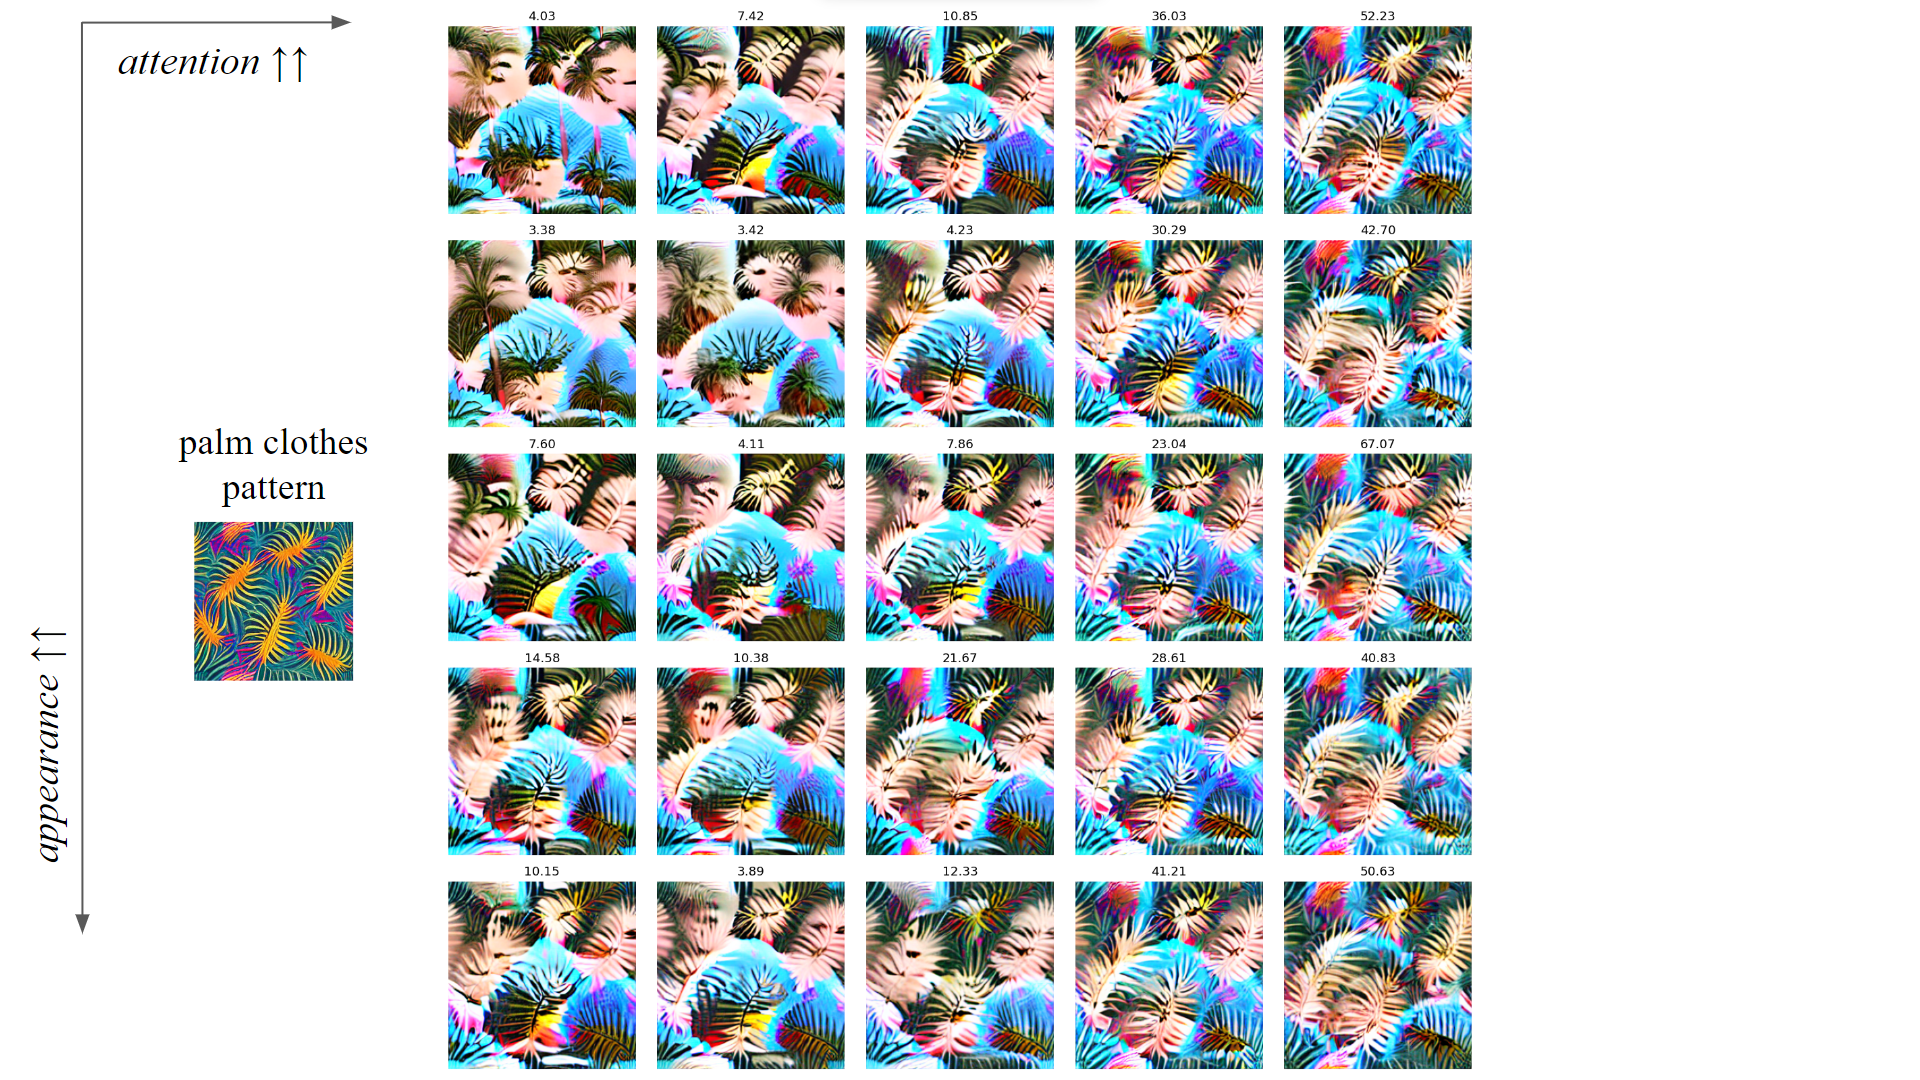
\includegraphics[clip, width=\columnwidth]{figures/fix_palm.png}\label{fix_palm}
}\hfill
\subfloat[``Space clothes pattern''.]{
  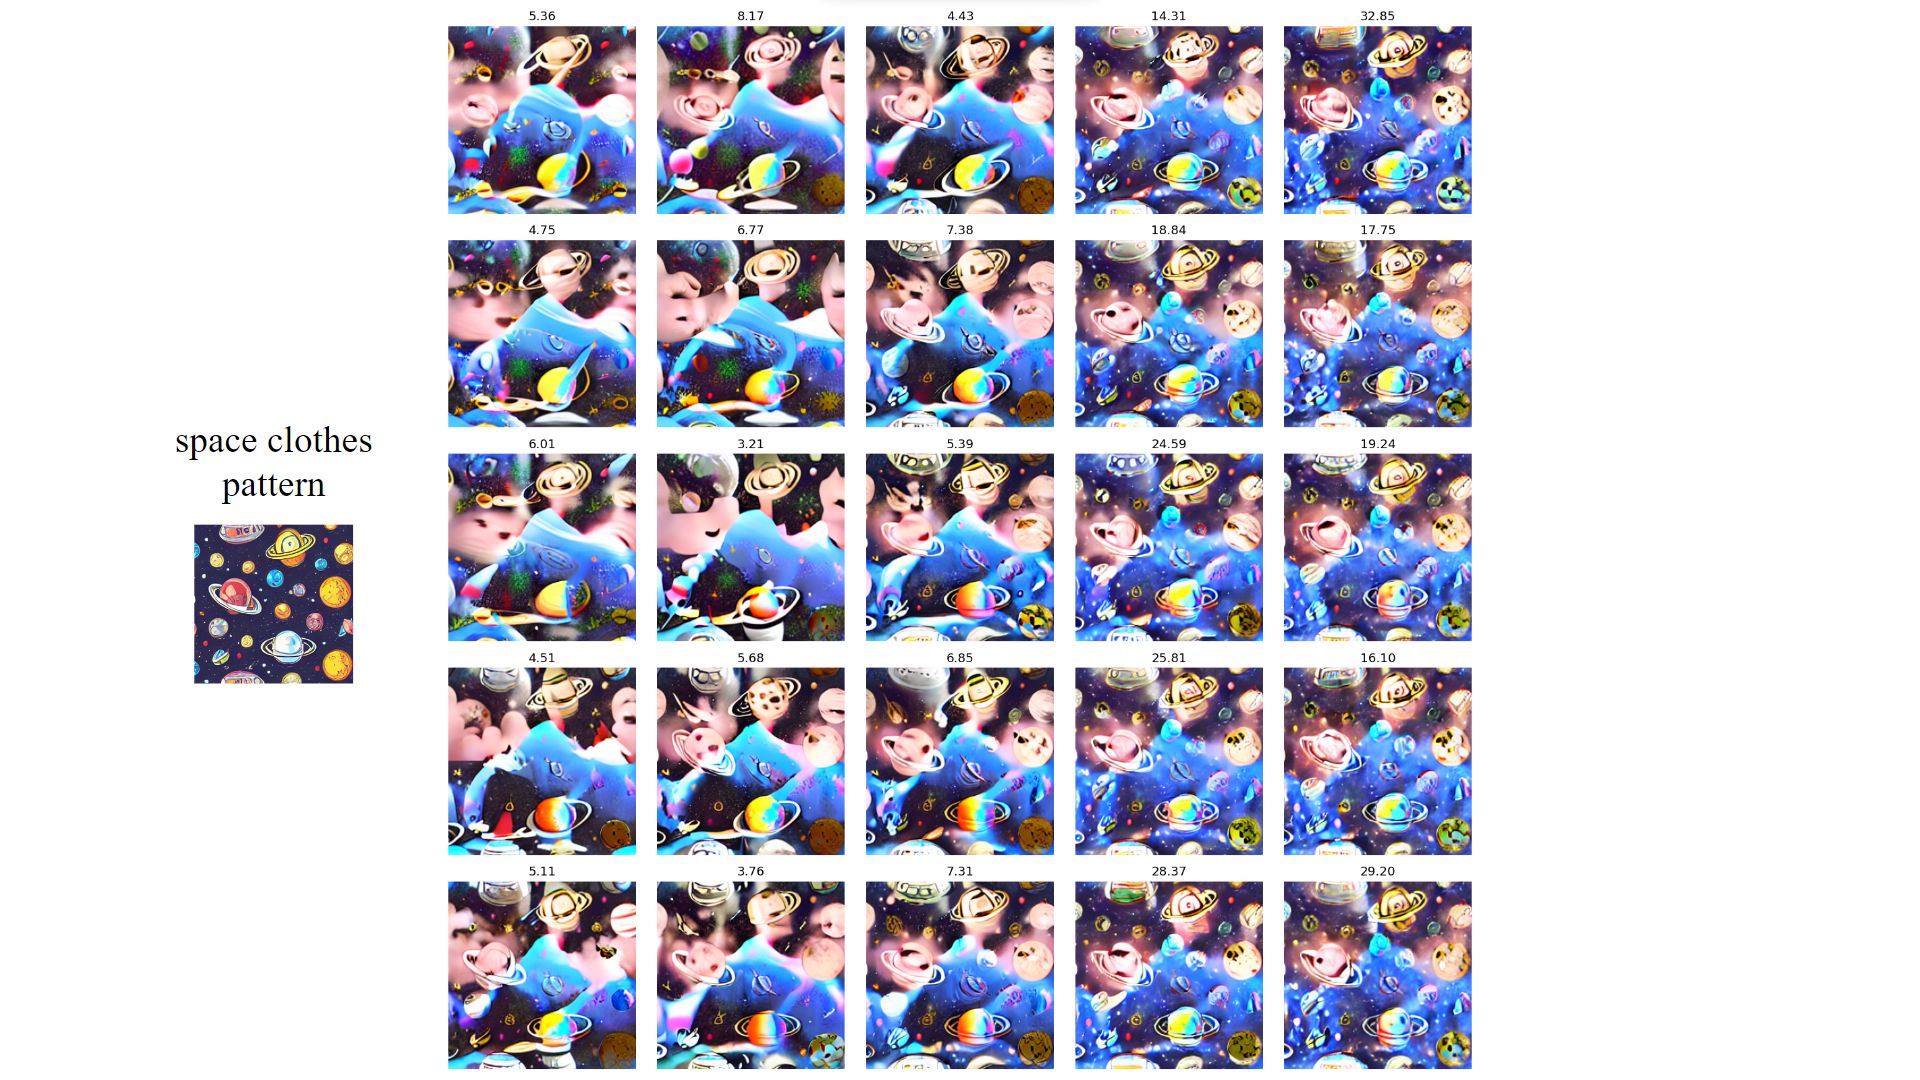
\includegraphics[clip, width=\columnwidth]{figures/fix_space.png}\label{fix_space}
}
\caption{Generations for the same adversarial scheduler with different strength of $s^{at}$ and $s^{ap}$ coefficients.}\label{fix_ex}
\end{figure}

Figure~\ref{fix_ex} shows how the trade-off between adversarial effectiveness and resemblance to the original image by varying attention and appearance constraint coefficients for two prompts, ``palm clothes pattern'' (Figure~\ref{fix_palm}) and ``space clothes pattern'' (Figure~\ref{fix_space}).

In the left part of both figures, we can see the non-adversarial versions for the prompts.

Appearance constraint coefficient $s^{ap}$ increases along the $y$ axis (top to bottom direction), while the self-attention constraint coefficient $s^{at}$ increases along the $x$ axis (left to right direction), so the last images in the last rows are the closest to their respective non-adversarial images, but also have the lowest adversarial effects.
While the resemblance to the non-adversarial pictures increases along both axes, we can see that self-attention constraint is indeed more effective for the same coefficients.

Sadly, we also notice that luck plays a visible part in the results since the AP does not change consistently.
However, considering the fact that we only generated the images for 256 steps and used a weak SD model but managed to obtain good APs nevertheless, the method looks very promising.
The AP is calculated in the digital world scenarios, but the patches are likely to be effective in the real physical world if the AP is at least lower than 7, and both prompts have relatively natural generations that satisfy that requirement. 

\subsection{Different Prompts}

TODO maybe best results for around 5 random prompts, and also with different prompt extensions

\subsection{Real Images}

TODO we can give the model real images, use ddim inversion to obtain latents and work with them (or perhaps phantom trajectories like in self-guidance paper?)

\subsection{Physical Results}

\paragraph{Patches}

\begin{figure}[htp]
\subfloat[``Space clothes pattern'' prompt, AP 12.]{
  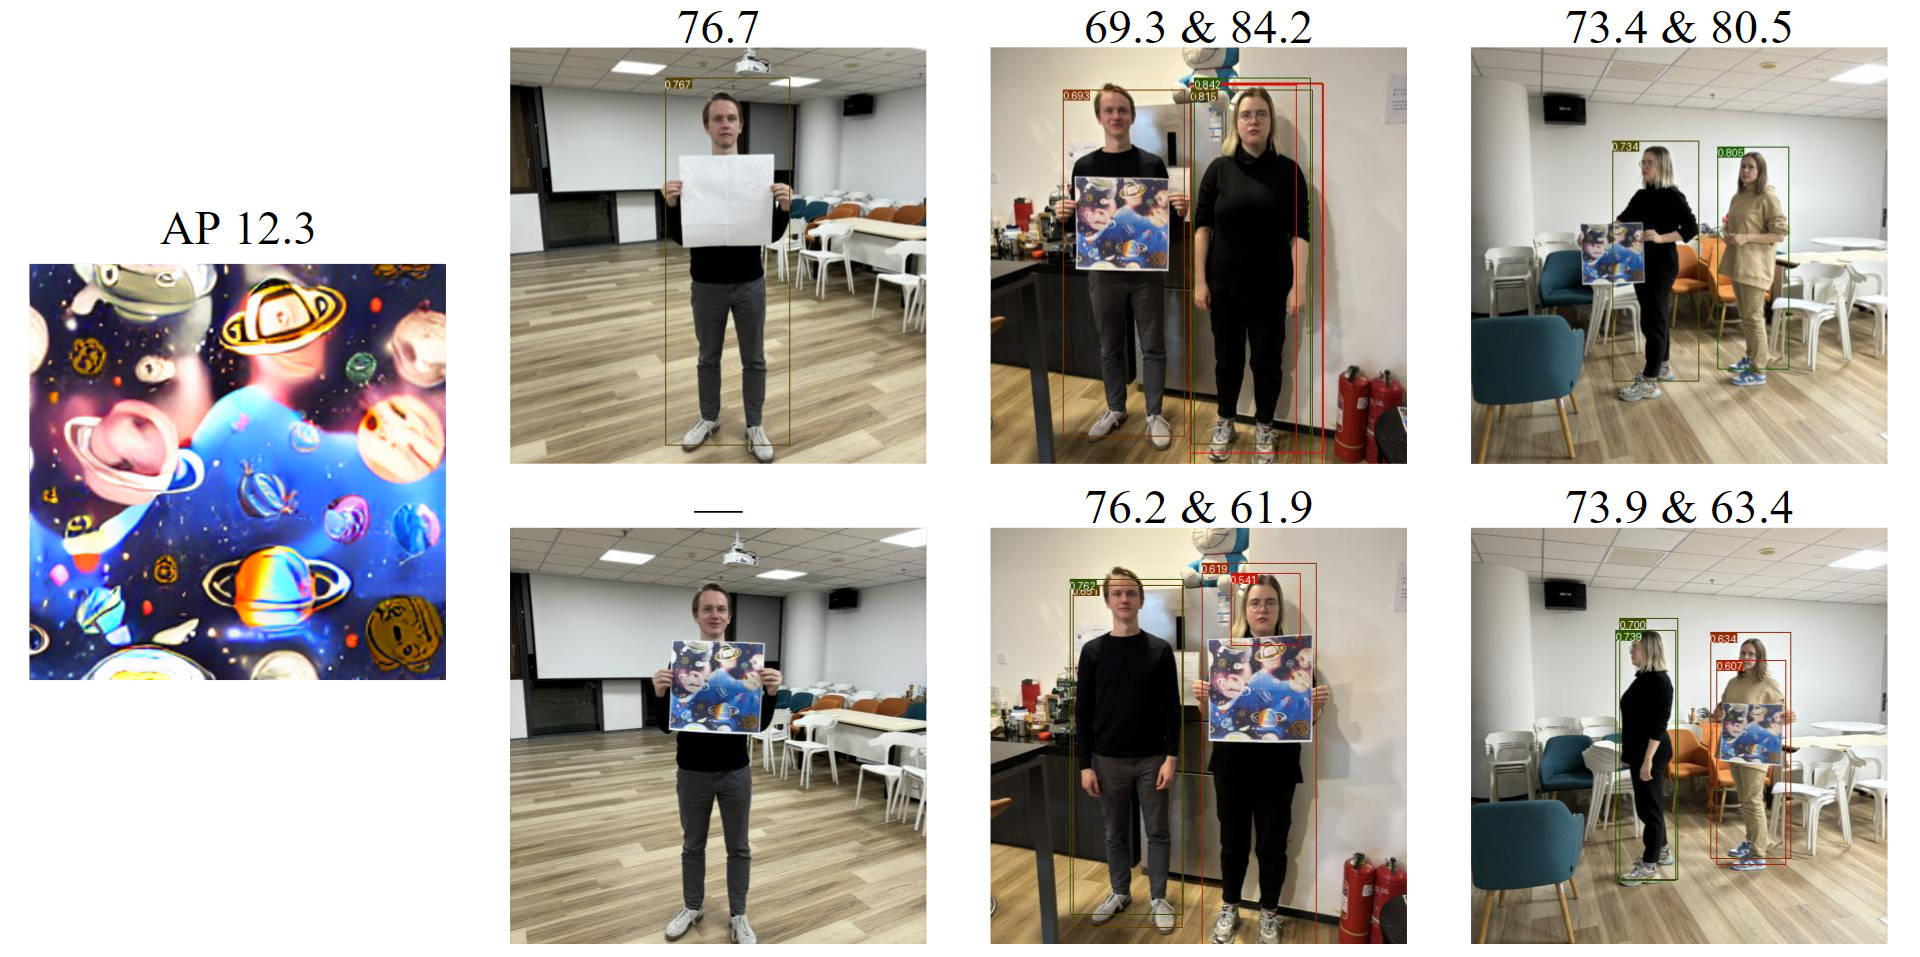
\includegraphics[clip, width=0.9\textwidth]{figures/phys_patch_space1.png}\label{physical_patch_space1}
}\hfill
\subfloat[``Space clothes pattern'' prompt, AP 4.]{
  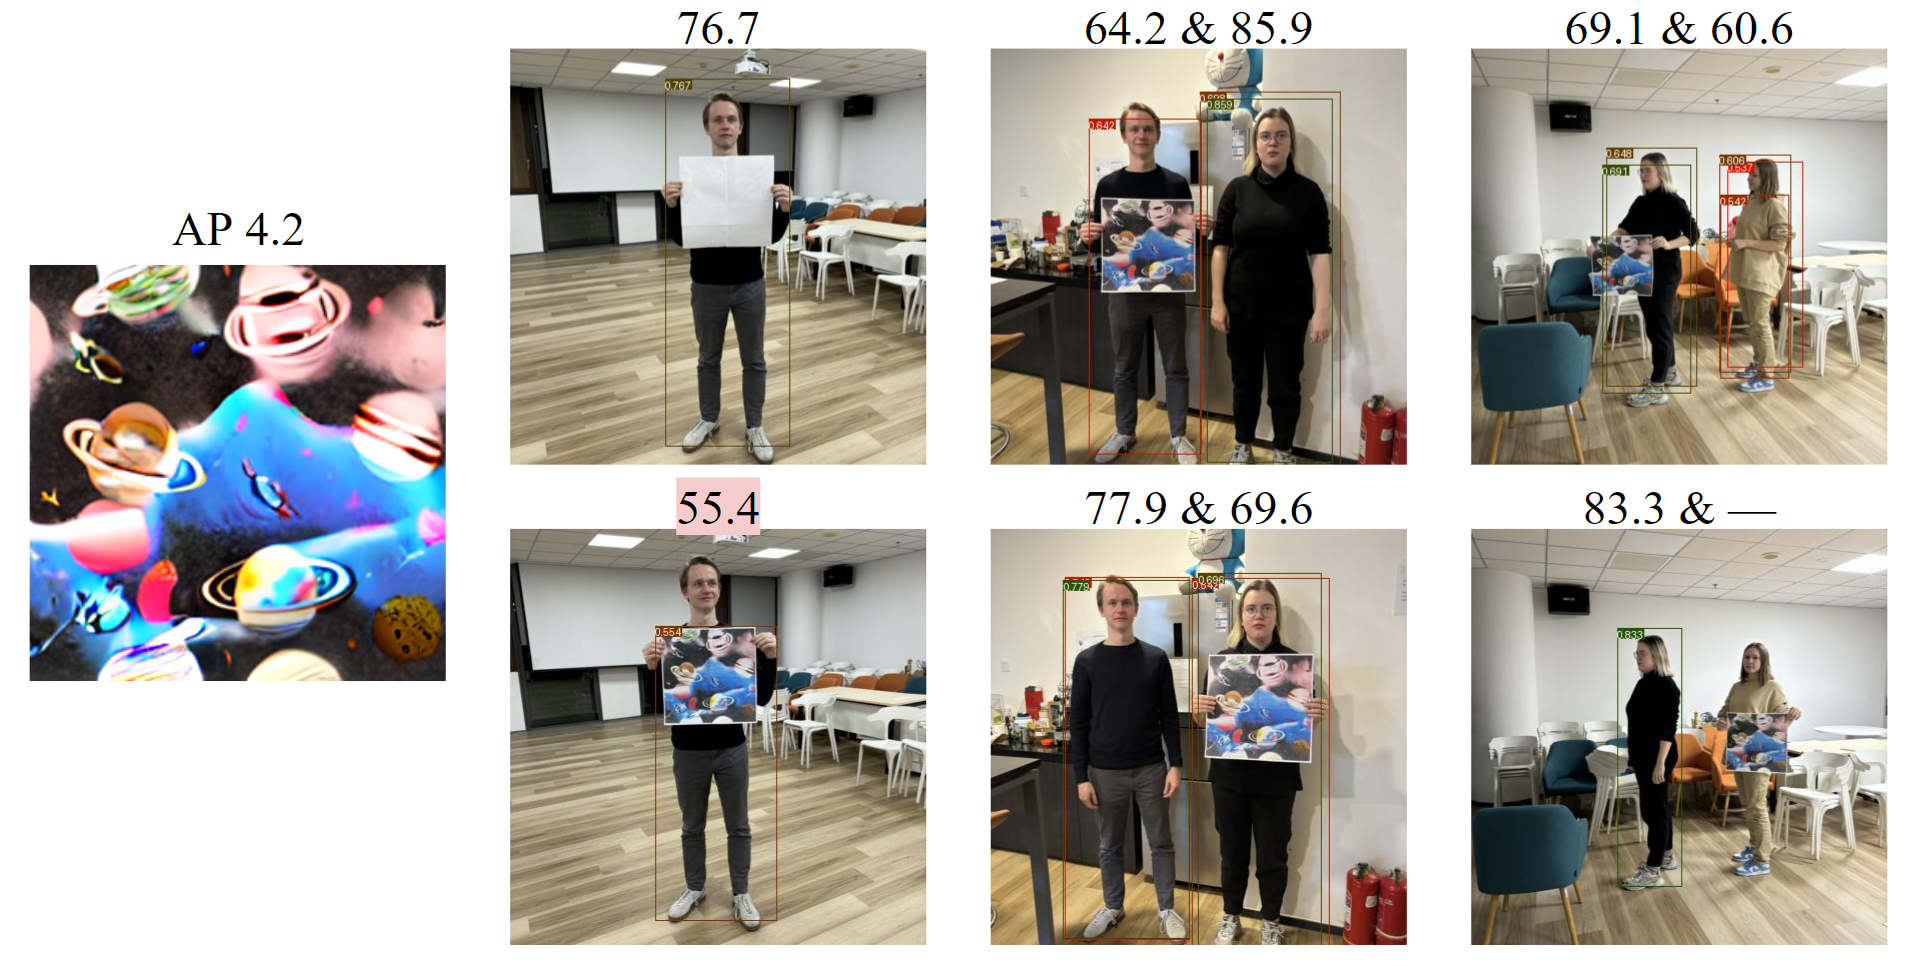
\includegraphics[clip, width=0.9\textwidth]{figures/phys_patch_space2.png}\label{physical_patch_space2}
}\hfill
\subfloat[``Flower clothes pattern'' prompt, AP 57.]{
  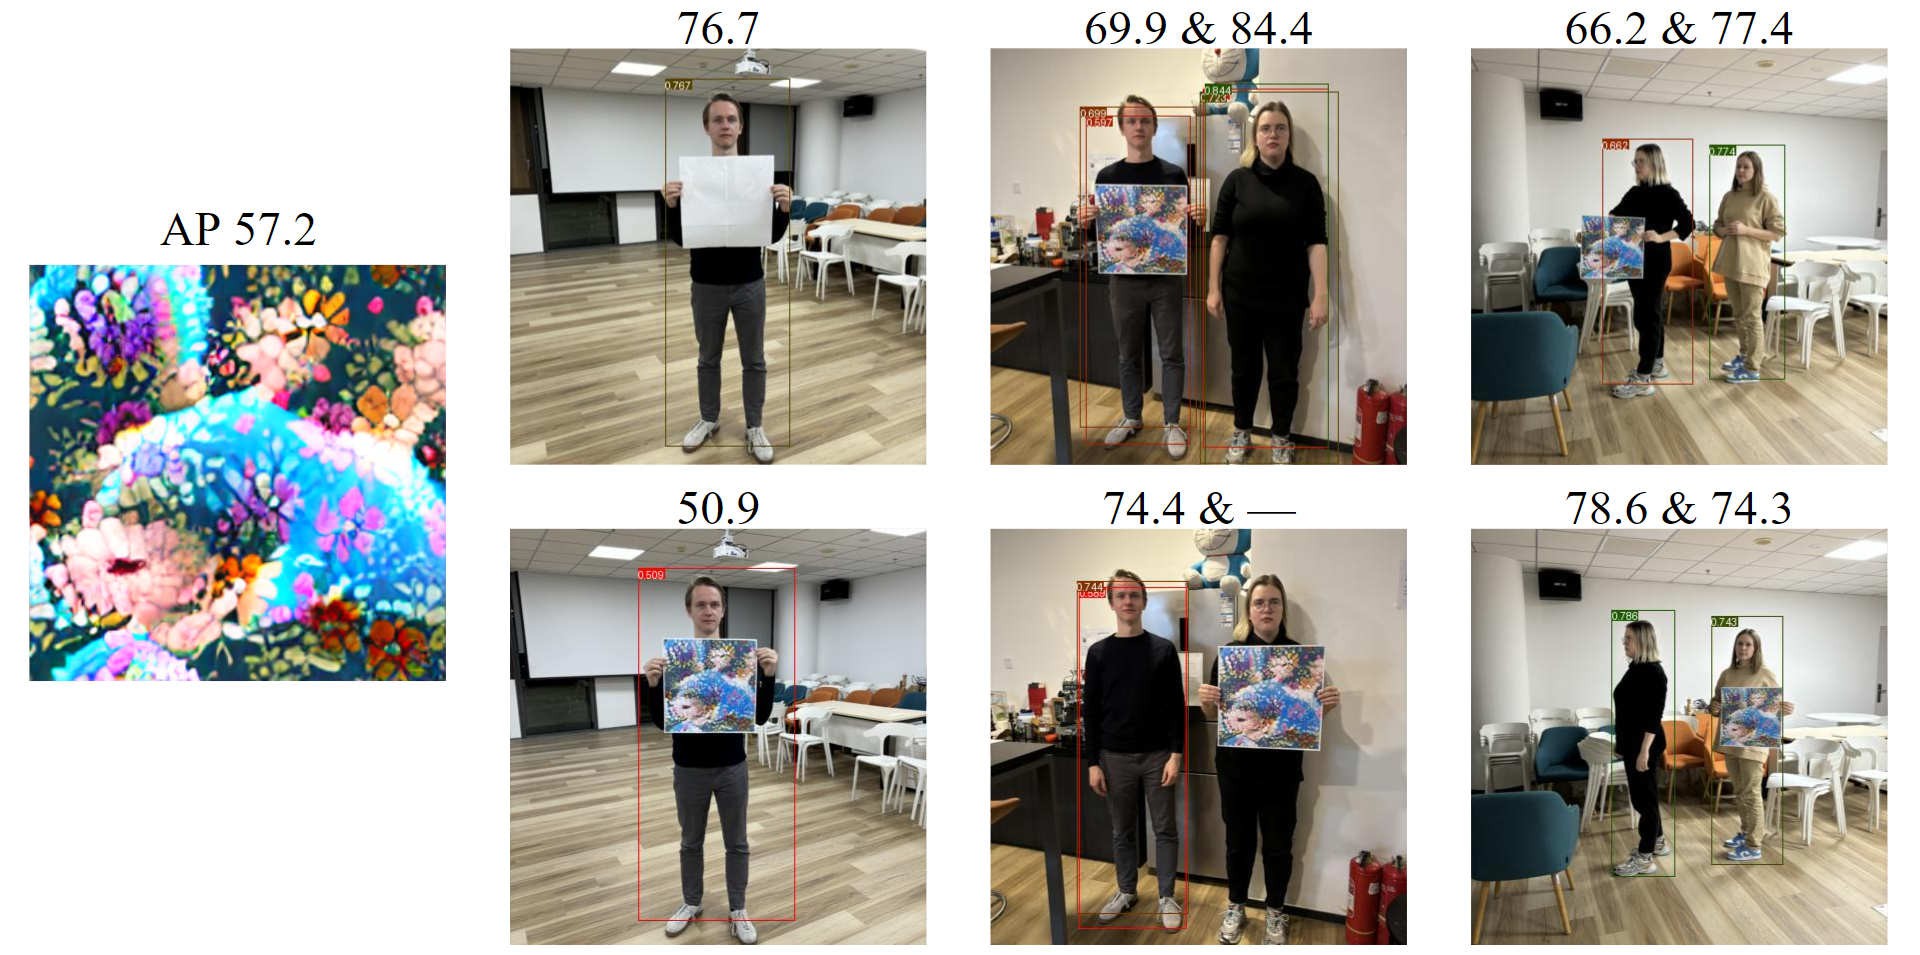
\includegraphics[clip, width=0.9\textwidth]{figures/phys_patch_flower.png}\label{physical_patch_flower}
}
\caption{Physical results with generations as patches trained with the 3D pipeline.}\label{physical_patches}
\end{figure}
 
Evaluation of physical results is rather challenging, mainly because printing actual clothes, taking videos with them, and then manually labelling all the data is very time-consuming and expensive.
Firstly, we need to ensure that the generated patterns actually work by, for example, only printing them as patches and checking their effectiveness in several settings. 
Examples of this approach can be found in Figure~\ref{physical_patches}.

TODO desc

\paragraph{Clothes}

TODO?

\section{Comparison Against Baseline Methods}

TODO for this, we need to switch to yolo3 


% \section{数学符号}

% 中文论文的数学符号默认遵循 GB/T 3102.11—1993《物理科学和技术中使用的数学符号》
% \footnote{原 GB 3102.11—1993,自 2017 年 3 月 23 日起,该标准转为推荐性标准。}。
% 该标准参照采纳 ISO 31-11:1992 \footnote{目前已更新为 ISO 80000-2:2019。},
% 但是与 \TeX{} 默认的美国数学学会(AMS)的符号习惯有所区别。
% 具体地来说主要有以下差异:
% \begin{enumerate}
%   \item 大写希腊字母默认为斜体,如
%     \begin{equation*}
%       \Gamma \Delta \Theta \Lambda \Xi \Pi \Sigma \Upsilon \Phi \Psi \Omega.
%     \end{equation*}
%     注意有限增量符号 $\increment$ 固定使用正体,模板提供了 \cs{increment} 命令。
%   \item 小于等于号和大于等于号使用倾斜的字形 $\le$、$\ge$。
%   \item 积分号使用正体,比如 $\int$、$\oint$。
%   \item
%     偏微分符号 $\partial$ 使用正体。
%   \item
%     省略号 \cs{dots} 按照中文的习惯固定居中,比如
%     \begin{equation*}
%       1, 2, \dots, n \quad 1 + 2 + \dots + n.
%     \end{equation*}
%   \item
%     实部 $\Re$ 和虚部 $\Im$ 的字体使用罗马体。
% \end{enumerate}

% 以上数学符号样式的差异可以在模板中统一设置。
% 另外国标还有一些与 AMS 不同的符号使用习惯,需要用户在写作时进行处理:
% \begin{enumerate}
%   \item 数学常数和特殊函数名用正体,如
%     \begin{equation*}
%       \uppi = 3.14\dots; \quad
%       \symup{i}^2 = -1; \quad
%       \symup{e} = \lim_{n \to \infty} \left( 1 + \frac{1}{n} \right)^n.
%     \end{equation*}
%   \item 微分号使用正体,比如 $\dif y / \dif x$。
%   \item 向量、矩阵和张量用粗斜体(\cs{symbf}),如 $\symbf{x}$、$\symbf{\Sigma}$、$\symbfsf{T}$。
%   \item 自然对数用 $\ln x$ 不用 $\log x$。
% \end{enumerate}


% 英文论文的数学符号使用 \TeX{} 默认的样式。
% 如果有必要,也可以通过设置 \verb|math-style| 选择数学符号样式。

% 关于量和单位推荐使用
% \href{http://mirrors.ctan.org/macros/latex/contrib/siunitx/siunitx.pdf}{\pkg{siunitx}}
% 宏包,
% 可以方便地处理希腊字母以及数字与单位之间的空白,
% 比如:
% \SI{6.4e6}{m},
% \SI{9}{\micro\meter},
% \si{kg.m.s^{-1}},
% \SIrange{10}{20}{\degreeCelsius}。



% \section{数学公式}

% 数学公式可以使用 \env{equation} 和 \env{equation*} 环境。
% 注意数学公式的引用应前后带括号,通常使用 \cs{eqref} 命令,比如式\eqref{eq:example}。
% \begin{equation}
%   \frac{1}{2 \uppi \symup{i}} \int_\gamma f = \sum_{k=1}^m n(\gamma; a_k) \mathscr{R}(f; a_k).
%   \label{eq:example}
% \end{equation}

% 多行公式尽可能在“=”处对齐,推荐使用 \env{align} 环境。
% \begin{align}
%   a & = b + c + d + e \\
%     & = f + g
% \end{align}



% \section{数学定理}

% 定理环境的格式可以使用 \pkg{amsthm} 或者 \pkg{ntheorem} 宏包配置。
% 用户在导言区载入这两者之一后,模板会自动配置 \env{thoerem}、\env{proof} 等环境。

% \begin{theorem}[Lindeberg--Lévy 中心极限定理]
%   设随机变量 $X_1, X_2, \dots, X_n$ 独立同分布, 且具有期望 $\mu$ 和有限的方差 $\sigma^2 \ne 0$,
%   记 $\bar{X}_n = \frac{1}{n} \sum_{i+1}^n X_i$,则
%   \begin{equation}
%     \lim_{n \to \infty} P \left(\frac{\sqrt{n} \left( \bar{X}_n - \mu \right)}{\sigma} \le z \right) = \Phi(z),
%   \end{equation}
%   其中 $\Phi(z)$ 是标准正态分布的分布函数。
% \end{theorem}
% \begin{proof}
%   Trivial.
% \end{proof}

% 同时模板还提供了 \env{assumption}、\env{definition}、\env{proposition}、
% \env{lemma}、\env{theorem}、\env{axiom}、\env{corollary}、\env{exercise}、
% \env{example}、\env{remar}、\env{problem}、\env{conjecture} 这些相关的环境。
